% Seminar 2: Classical distributions and stylised facts
% Statistics of Financial Markets -- Bachelor's programme, Bucharest University of Economic Studies
% GENERATED by latex/build_seminar2.py -- edit the generator, not this file.
% Student version by default; the instructor version is the *_solutions.tex wrapper.
\makeatletter\@ifundefined{ifsolutions}{\expandafter\newif\csname ifsolutions\endcsname}{}\makeatother

\newcommand{\coursename}{Statistics of Financial Markets}
% Preambul comun SFM -- Statistica piețelor financiare / Statistics of Financial Markets (Beamer, 16:9)
% Același design ca MFM. Înainte de % Preambul comun SFM -- Statistica piețelor financiare / Statistics of Financial Markets (Beamer, 16:9)
% Același design ca MFM. Înainte de % Preambul comun SFM -- Statistica piețelor financiare / Statistics of Financial Markets (Beamer, 16:9)
% Același design ca MFM. Înainte de \input{../../latex/preamble} se definește
%   \newcommand{\coursename}{Statistics of Financial Markets}      (EN)
%   \newcommand{\coursename}{Statistica piețelor financiare}       (RO)  și  \def\sfmlang{ro}
% Fișierele .tex se află în EN/Courses, EN/Seminars, RO/Cursuri, RO/Seminarii (două niveluri sub rădăcină).
% Deck-urile sînt generate de latex/build_chapterN.py / build_seminarN.py (vezi latex/sfm_build.py).

\documentclass[9pt, aspectratio=169, t]{beamer}
\providecommand{\coursename}{Statistics of Financial Markets}

% Ensure content fits on slides
\setbeamersize{text margin left=8mm, text margin right=8mm}

%=============================================================================
% THEME AND STYLE CONFIGURATION
%=============================================================================
\usetheme{default}
% Using default theme for clean header/footer control

% Color Palette (matching Redispatch PDF)
\definecolor{MainBlue}{RGB}{26, 58, 110}
\definecolor{AccentBlue}{RGB}{26, 58, 110}
\definecolor{IDAred}{RGB}{205, 0, 0}
\definecolor{DarkGray}{RGB}{51, 51, 51}
\definecolor{MediumGray}{RGB}{128, 128, 128}
\definecolor{LightGray}{RGB}{248, 248, 248}
\definecolor{VeryLightGray}{RGB}{235, 235, 235}
\definecolor{KeynoteGray}{RGB}{218, 218, 218}
\definecolor{SectionGray}{RGB}{120, 120, 120}
\definecolor{FooterGray}{RGB}{100, 100, 100}
\definecolor{Crimson}{RGB}{220, 53, 69}
\definecolor{Forest}{RGB}{46, 125, 50}
\definecolor{Amber}{RGB}{181, 133, 63}
\definecolor{Orange}{RGB}{230, 126, 34}
\definecolor{Purple}{RGB}{142, 68, 173}

% Gradient background (exact Keynote 315° gradient: white to RGB 218,218,218)
\setbeamertemplate{background}{%
    \begin{tikzpicture}[remember picture, overlay]
        \shade[shading=axis, shading angle=315,
        top color=white, bottom color=KeynoteGray]
        (current page.south west) rectangle (current page.north east);
    \end{tikzpicture}%
}
% Fallback solid color for compatibility
\setbeamercolor{background canvas}{bg=}

\setbeamercolor{palette primary}{bg=MainBlue, fg=white}
\setbeamercolor{palette secondary}{bg=MainBlue!85, fg=white}
\setbeamercolor{palette tertiary}{bg=MainBlue!70, fg=white}
\setbeamercolor{structure}{fg=MainBlue}
\setbeamercolor{title}{fg=IDAred}
\setbeamercolor{frametitle}{fg=IDAred, bg=}
\setbeamercolor{block title}{bg=MainBlue, fg=white}
\setbeamercolor{block body}{bg=VeryLightGray, fg=DarkGray}
\setbeamercolor{block title alerted}{bg=Crimson, fg=white}
\setbeamercolor{block body alerted}{bg=Crimson!8, fg=DarkGray}
\setbeamercolor{block title example}{bg=Forest, fg=white}
\setbeamercolor{block body example}{bg=Forest!8, fg=DarkGray}
\setbeamercolor{item}{fg=MainBlue}

% Footer colors (override Madrid theme blue)
\setbeamercolor{author in head/foot}{fg=FooterGray, bg=}
\setbeamercolor{title in head/foot}{fg=FooterGray, bg=}
\setbeamercolor{date in head/foot}{fg=FooterGray, bg=}
\setbeamercolor{section in head/foot}{fg=FooterGray, bg=}
\setbeamercolor{subsection in head/foot}{fg=FooterGray, bg=}

% Bullet styles (apply everywhere including blocks)
\setbeamertemplate{itemize item}{\color{MainBlue}$\boxdot$}
\setbeamertemplate{itemize subitem}{\color{MainBlue}$\blacktriangleright$}
\setbeamertemplate{itemize subsubitem}{\color{MainBlue}\tiny$\bullet$}
\setbeamertemplate{itemize/enumerate body begin}{\normalsize}
\setbeamertemplate{itemize/enumerate subbody begin}{\normalsize}

% Item spacing - compact style
\setlength{\leftmargini}{10pt}       % Level 1: minimal indent
\setlength{\leftmarginii}{10pt}      % Level 2: minimal additional indent
% Compact list spacing (zero extra space before/after lists in blocks)
\makeatletter
\def\@listi{\leftmargin\leftmargini \topsep 0pt \parsep 0pt \itemsep 0pt}
\def\@listii{\leftmargin\leftmarginii \topsep 0pt \parsep 0pt \itemsep 0pt}
\makeatother

\setbeamertemplate{navigation symbols}{}

%=============================================================================
% CUSTOM HEADLINE
%=============================================================================
\setbeamertemplate{headline}{%
    \vskip10pt%
    \hbox to \paperwidth{%
        \hskip0.5cm%
        {\small\color{FooterGray}\renewcommand{\hyperlink}[2]{##2}\insertsectionhead}%
        \hfill%
        \textcolor{FooterGray}{\small\insertframenumber}%
        \hskip0.5cm%
    }%
    \vskip4pt%
    {\color{FooterGray}\hrule height 0.4pt}%
}

%=============================================================================
% CUSTOM FOOTER
%=============================================================================
\usepackage{fontawesome5}

\setbeamertemplate{footline}{%
    {\color{FooterGray}\hrule height 0.4pt}%
    \vskip4pt%
    \hbox to \paperwidth{%
        \hskip0.5cm%
        \textcolor{FooterGray}{\small\coursename}%
        \hfill%
        \raisebox{-0.1em}{%
            \begin{tikzpicture}[x=0.08em, y=0.08em, line width=0.4pt]
                \draw[FooterGray] (0,3) -- (1,4) -- (2,3.5) -- (3,5) -- (4,4) -- (5,6) -- (6,5.5) -- (7,4) -- (8,5) -- (9,7) -- (10,6) -- (11,5) -- (12,6.5) -- (13,8) -- (14,7) -- (15,6) -- (16,7.5) -- (17,9) -- (18,8) -- (19,7) -- (20,8.5) -- (21,10) -- (22,9) -- (23,8) -- (24,9.5);
            \end{tikzpicture}%
        }%
        \hskip0.5cm%
    }%
    \vskip6pt%
}

%=============================================================================
% PACKAGES
%=============================================================================
\usepackage[utf8]{inputenc}
\DeclareUnicodeCharacter{03B1}{\ensuremath{\alpha}}
\usepackage[T1]{fontenc}
\usepackage{amsmath, amssymb, amsthm}
\usepackage{mathtools}
\usepackage{bm}
\usepackage{tikz}
\usetikzlibrary{arrows.meta, positioning, shapes, calc, decorations.pathreplacing, shadings}
\usepackage{booktabs}
\usepackage{multirow}
\usepackage{array}
\usepackage{graphicx}
\usepackage{hyperref}
\usepackage{colortbl}
\usepackage{listings}
\lstset{language=Python, basicstyle=\ttfamily\scriptsize, keywordstyle=\color{MainBlue}\bfseries,
  commentstyle=\color{Forest}, stringstyle=\color{Crimson}, breaklines=true,
  frame=none, backgroundcolor=\color{VeryLightGray}, xleftmargin=2mm}
\hypersetup{colorlinks=true, linkcolor=MainBlue, urlcolor=MainBlue}
\graphicspath{{../../logos/}{../../charts/}{../../photos/}}
\usepackage{xcolor}
\hfuzz=2pt  % Suppress tiny overfull warnings (<2pt)
\vfuzz=2pt  % Suppress tiny vertical overfull warnings (<2pt)

%=============================================================================
% QUANTLET COMMANDS
%   \quantlet{<displayed name>}{<url>}       (generic, compatible with the older SFM decks)
%   \sfmquantlet{Ch_05}{SFM_ch5_garch}       -> https://github.com/danpele/SFM/tree/main/Quantlets/Ch_05/SFM_ch5_garch
%   \qlurl{<folder>} is defined per chapter by the generator (Quantlets/Ch_NN/<folder>)
%=============================================================================
\newcommand{\sfmrepo}{https://github.com/danpele/SFM}
\newcommand{\sfmqlbase}{https://github.com/danpele/SFM/tree/main/Quantlets}
\newcommand{\quantlet}[2]{%
    \hfill\href{#2}{%
        \raisebox{-0.15em}{
\includegraphics[height=0.7em]{ql_logo.png}}%
        \textcolor{MainBlue}{\tiny\ #1}%
    }%
}
\newcommand{\sfmquantlet}[2]{\quantlet{\detokenize{#2}}{\sfmqlbase/#1/#2}}

%=============================================================================
% NOTEBOOKS (Google Colab)
%   \colaburl{notebooks/EN/chapter5_seminar_notebook.ipynb} -> the Colab link of a file in the SFM repo
%   \nb: the chapter notebook (each seminar deck redefines it with \renewcommand)
%=============================================================================
\newcommand{\colaburl}[1]{https://colab.research.google.com/github/danpele/SFM/blob/main/#1}
\newcommand{\nb}{https://colab.research.google.com/github/danpele/SFM/tree/main/notebooks/EN}
\newcommand{\nbname}{notebooks/EN}

%=============================================================================
% SLIDE HELPERS (used by the generators; the same as in MFM)
%=============================================================================
% local font size for list bodies (the preamble forces \normalsize)
\newcommand{\itemsize}[1]{\setbeamertemplate{itemize/enumerate body begin}{#1}\setbeamertemplate{itemize/enumerate subbody begin}{#1}}
\newcommand{\intitle}[1]{{\hypersetup{urlcolor=white}#1}}   % white links inside coloured title bars
\newcommand{\imgcap}[1]{{\scriptsize #1}\\[0.5mm]}          % caption under a photo
\newcommand{\imgcredit}[2]{{\tiny\color{FooterGray}\href{#1}{#2}}}   % image credit: source URL, author/licence
\newcommand{\aiprompt}[1]{{\ttfamily\color{MainBlue}#1}}     % a prompt to an AI assistant

%=============================================================================
% SEMINARS: student version by default; the instructor wrapper *_solutions.tex sets \solutionstrue
%=============================================================================
\makeatletter\@ifundefined{ifsolutions}{\expandafter\newif\csname ifsolutions\endcsname}{}\makeatother
\newcommand{\solonly}[1]{\ifsolutions #1\fi}
\newcommand{\propsub}{\ifsolutions\else\framesubtitle{\ifdefined\sfmlang Rezolvarea se discută la seminar\else Solution discussed in class\fi}\fi}

%=============================================================================
% APPENDIX AND CHAPTER LINKS (latex/appendix_links.py writes the calls; it also re-declares these
% macros before \begin{document}, so the decks compile with or without this preamble block)
%=============================================================================
\providecommand{\sfmapplink}[3]{\hypertarget{#2}{}\hyperlink{#1}{\beamergotobutton{#3}}}
\providecommand{\sfmappback}[2]{\begin{tikzpicture}[remember picture,overlay]\node[anchor=south east] at ([xshift=-3mm,yshift=7mm]current page.south east){\hyperlink{#1}{\beamerreturnbutton{#2}}};\end{tikzpicture}}
\providecommand{\sfmchlink}[2]{\href{#1}{#2}}
\providecommand{\sfmchlinkt}[2]{\href{#1}{\usebeamercolor[fg]{frametitle}#2}}

%=============================================================================
% QUANTINAR COMMAND: link către un curs Quantinar (subiecte avansate)
%=============================================================================
\newcommand{\quantinar}[2]{%
    \href{#2}{%
        \raisebox{-0.15em}{
\includegraphics[height=0.8em]{qr_logo.png}}%
        \textcolor{MainBlue}{\scriptsize\ #1}%
    }%
}

%=============================================================================
% CUSTOM TITLE PAGE
%=============================================================================
\defbeamertemplate*{title page}{hybrid}[1][]
{
    \vspace{0.2cm}
    % Logos row - top header (with clickable links)
    \begin{center}
        \href{https://www.ase.ro}{
\includegraphics[height=1.0cm]{ase_logo.png}}\hspace{0.3cm}%
        \href{https://theida.net}{
\includegraphics[height=1.0cm]{ida_logo.png}}\hspace{0.3cm}%
        \href{https://blockchain-research-center.com}{
\includegraphics[height=1.0cm]{brc_logo.png}}\hspace{0.3cm}%
        \href{https://www.ai4efin.ase.ro}{
\includegraphics[height=1.0cm]{ai4efin_logo.png}}\hspace{0.3cm}%
        \href{https://ipe.ro/new}{
\includegraphics[height=1.0cm]{acad_logo.png}}\hspace{0.3cm}%
        \href{https://www.digital-finance-msca.com}{
\includegraphics[height=1.0cm]{msca_logo.png}}%
    \end{center}

    \vspace{0.6cm}

    % Main title with Q logos on sides (with clickable links)
    \begin{center}
        \begin{minipage}{0.1\textwidth}
            \centering
            \href{https://quantlet.com}{
\includegraphics[height=1.1cm]{ql_logo.png}}
        \end{minipage}%
        \begin{minipage}{0.78\textwidth}
            \centering
            {\LARGE\bfseries\usebeamercolor[fg]{title}\inserttitle}

            \vspace{0.3cm}

            {\usebeamerfont{subtitle}\usebeamercolor[fg]{title}\insertsubtitle}
        \end{minipage}%
        \begin{minipage}{0.1\textwidth}
            \centering
            \href{https://quantinar.com}{
\includegraphics[height=1.1cm]{qr_logo.png}}
        \end{minipage}
    \end{center}

    \vspace{0.6cm}

    % Authors (left aligned)
    \hspace{0.5cm}{\usebeamerfont{author}\insertauthor}

    \vspace{0.3cm}

    % Institute/Affiliations (left aligned)
    \hspace{0.5cm}\begin{minipage}[t]{0.9\textwidth}
        \raggedright\small\insertinstitute
    \end{minipage}
}

%=============================================================================
% THEOREM ENVIRONMENTS
%=============================================================================
\theoremstyle{definition}
\setbeamertemplate{theorems}[numbered]
\ifdefined\sfmlang
\newtheorem{defn}{Definiție}
\newtheorem{thm}{Teoremă}
\newtheorem{prop}{Propoziție}
\newtheorem{rmk}{Observație}
\else
\newtheorem{defn}{Definition}
\newtheorem{thm}{Theorem}
\newtheorem{prop}{Proposition}
\newtheorem{rmk}{Remark}
\fi

%=============================================================================
% CENTRED MINIPAGE (no extra vertical space)
%=============================================================================
\newenvironment{cminipage}[1]{%
    \par\noindent\hfill\begin{minipage}{#1}\ignorespaces
}{%
    \end{minipage}\hfill\null\par
}

%=============================================================================
% CUSTOM COMMANDS
%=============================================================================
\newcommand{\E}{\mathbb{E}}
\newcommand{\Var}{\text{Var}}
\newcommand{\Cov}{\text{Cov}}
\newcommand{\Corr}{\text{Corr}}
\newcommand{\R}{\mathbb{R}}
\newcommand{\N}{\mathbb{N}}
\newcommand{\Z}{\mathbb{Z}}
\newcommand{\B}{\mathbf{B}}
\newcommand{\imark}{\textcolor{MainBlue}{\textbullet}}
\newcommand{\RMSE}{\text{RMSE}}
\newcommand{\MAE}{\text{MAE}}
\newcommand{\MAPE}{\text{MAPE}}

 se definește
%   \newcommand{\coursename}{Statistics of Financial Markets}      (EN)
%   \newcommand{\coursename}{Statistica piețelor financiare}       (RO)  și  \def\sfmlang{ro}
% Fișierele .tex se află în EN/Courses, EN/Seminars, RO/Cursuri, RO/Seminarii (două niveluri sub rădăcină).
% Deck-urile sînt generate de latex/build_chapterN.py / build_seminarN.py (vezi latex/sfm_build.py).

\documentclass[9pt, aspectratio=169, t]{beamer}
\providecommand{\coursename}{Statistics of Financial Markets}

% Ensure content fits on slides
\setbeamersize{text margin left=8mm, text margin right=8mm}

%=============================================================================
% THEME AND STYLE CONFIGURATION
%=============================================================================
\usetheme{default}
% Using default theme for clean header/footer control

% Color Palette (matching Redispatch PDF)
\definecolor{MainBlue}{RGB}{26, 58, 110}
\definecolor{AccentBlue}{RGB}{26, 58, 110}
\definecolor{IDAred}{RGB}{205, 0, 0}
\definecolor{DarkGray}{RGB}{51, 51, 51}
\definecolor{MediumGray}{RGB}{128, 128, 128}
\definecolor{LightGray}{RGB}{248, 248, 248}
\definecolor{VeryLightGray}{RGB}{235, 235, 235}
\definecolor{KeynoteGray}{RGB}{218, 218, 218}
\definecolor{SectionGray}{RGB}{120, 120, 120}
\definecolor{FooterGray}{RGB}{100, 100, 100}
\definecolor{Crimson}{RGB}{220, 53, 69}
\definecolor{Forest}{RGB}{46, 125, 50}
\definecolor{Amber}{RGB}{181, 133, 63}
\definecolor{Orange}{RGB}{230, 126, 34}
\definecolor{Purple}{RGB}{142, 68, 173}

% Gradient background (exact Keynote 315° gradient: white to RGB 218,218,218)
\setbeamertemplate{background}{%
    \begin{tikzpicture}[remember picture, overlay]
        \shade[shading=axis, shading angle=315,
        top color=white, bottom color=KeynoteGray]
        (current page.south west) rectangle (current page.north east);
    \end{tikzpicture}%
}
% Fallback solid color for compatibility
\setbeamercolor{background canvas}{bg=}

\setbeamercolor{palette primary}{bg=MainBlue, fg=white}
\setbeamercolor{palette secondary}{bg=MainBlue!85, fg=white}
\setbeamercolor{palette tertiary}{bg=MainBlue!70, fg=white}
\setbeamercolor{structure}{fg=MainBlue}
\setbeamercolor{title}{fg=IDAred}
\setbeamercolor{frametitle}{fg=IDAred, bg=}
\setbeamercolor{block title}{bg=MainBlue, fg=white}
\setbeamercolor{block body}{bg=VeryLightGray, fg=DarkGray}
\setbeamercolor{block title alerted}{bg=Crimson, fg=white}
\setbeamercolor{block body alerted}{bg=Crimson!8, fg=DarkGray}
\setbeamercolor{block title example}{bg=Forest, fg=white}
\setbeamercolor{block body example}{bg=Forest!8, fg=DarkGray}
\setbeamercolor{item}{fg=MainBlue}

% Footer colors (override Madrid theme blue)
\setbeamercolor{author in head/foot}{fg=FooterGray, bg=}
\setbeamercolor{title in head/foot}{fg=FooterGray, bg=}
\setbeamercolor{date in head/foot}{fg=FooterGray, bg=}
\setbeamercolor{section in head/foot}{fg=FooterGray, bg=}
\setbeamercolor{subsection in head/foot}{fg=FooterGray, bg=}

% Bullet styles (apply everywhere including blocks)
\setbeamertemplate{itemize item}{\color{MainBlue}$\boxdot$}
\setbeamertemplate{itemize subitem}{\color{MainBlue}$\blacktriangleright$}
\setbeamertemplate{itemize subsubitem}{\color{MainBlue}\tiny$\bullet$}
\setbeamertemplate{itemize/enumerate body begin}{\normalsize}
\setbeamertemplate{itemize/enumerate subbody begin}{\normalsize}

% Item spacing - compact style
\setlength{\leftmargini}{10pt}       % Level 1: minimal indent
\setlength{\leftmarginii}{10pt}      % Level 2: minimal additional indent
% Compact list spacing (zero extra space before/after lists in blocks)
\makeatletter
\def\@listi{\leftmargin\leftmargini \topsep 0pt \parsep 0pt \itemsep 0pt}
\def\@listii{\leftmargin\leftmarginii \topsep 0pt \parsep 0pt \itemsep 0pt}
\makeatother

\setbeamertemplate{navigation symbols}{}

%=============================================================================
% CUSTOM HEADLINE
%=============================================================================
\setbeamertemplate{headline}{%
    \vskip10pt%
    \hbox to \paperwidth{%
        \hskip0.5cm%
        {\small\color{FooterGray}\renewcommand{\hyperlink}[2]{##2}\insertsectionhead}%
        \hfill%
        \textcolor{FooterGray}{\small\insertframenumber}%
        \hskip0.5cm%
    }%
    \vskip4pt%
    {\color{FooterGray}\hrule height 0.4pt}%
}

%=============================================================================
% CUSTOM FOOTER
%=============================================================================
\usepackage{fontawesome5}

\setbeamertemplate{footline}{%
    {\color{FooterGray}\hrule height 0.4pt}%
    \vskip4pt%
    \hbox to \paperwidth{%
        \hskip0.5cm%
        \textcolor{FooterGray}{\small\coursename}%
        \hfill%
        \raisebox{-0.1em}{%
            \begin{tikzpicture}[x=0.08em, y=0.08em, line width=0.4pt]
                \draw[FooterGray] (0,3) -- (1,4) -- (2,3.5) -- (3,5) -- (4,4) -- (5,6) -- (6,5.5) -- (7,4) -- (8,5) -- (9,7) -- (10,6) -- (11,5) -- (12,6.5) -- (13,8) -- (14,7) -- (15,6) -- (16,7.5) -- (17,9) -- (18,8) -- (19,7) -- (20,8.5) -- (21,10) -- (22,9) -- (23,8) -- (24,9.5);
            \end{tikzpicture}%
        }%
        \hskip0.5cm%
    }%
    \vskip6pt%
}

%=============================================================================
% PACKAGES
%=============================================================================
\usepackage[utf8]{inputenc}
\DeclareUnicodeCharacter{03B1}{\ensuremath{\alpha}}
\usepackage[T1]{fontenc}
\usepackage{amsmath, amssymb, amsthm}
\usepackage{mathtools}
\usepackage{bm}
\usepackage{tikz}
\usetikzlibrary{arrows.meta, positioning, shapes, calc, decorations.pathreplacing, shadings}
\usepackage{booktabs}
\usepackage{multirow}
\usepackage{array}
\usepackage{graphicx}
\usepackage{hyperref}
\usepackage{colortbl}
\usepackage{listings}
\lstset{language=Python, basicstyle=\ttfamily\scriptsize, keywordstyle=\color{MainBlue}\bfseries,
  commentstyle=\color{Forest}, stringstyle=\color{Crimson}, breaklines=true,
  frame=none, backgroundcolor=\color{VeryLightGray}, xleftmargin=2mm}
\hypersetup{colorlinks=true, linkcolor=MainBlue, urlcolor=MainBlue}
\graphicspath{{../../logos/}{../../charts/}{../../photos/}}
\usepackage{xcolor}
\hfuzz=2pt  % Suppress tiny overfull warnings (<2pt)
\vfuzz=2pt  % Suppress tiny vertical overfull warnings (<2pt)

%=============================================================================
% QUANTLET COMMANDS
%   \quantlet{<displayed name>}{<url>}       (generic, compatible with the older SFM decks)
%   \sfmquantlet{Ch_05}{SFM_ch5_garch}       -> https://github.com/danpele/SFM/tree/main/Quantlets/Ch_05/SFM_ch5_garch
%   \qlurl{<folder>} is defined per chapter by the generator (Quantlets/Ch_NN/<folder>)
%=============================================================================
\newcommand{\sfmrepo}{https://github.com/danpele/SFM}
\newcommand{\sfmqlbase}{https://github.com/danpele/SFM/tree/main/Quantlets}
\newcommand{\quantlet}[2]{%
    \hfill\href{#2}{%
        \raisebox{-0.15em}{
\includegraphics[height=0.7em]{ql_logo.png}}%
        \textcolor{MainBlue}{\tiny\ #1}%
    }%
}
\newcommand{\sfmquantlet}[2]{\quantlet{\detokenize{#2}}{\sfmqlbase/#1/#2}}

%=============================================================================
% NOTEBOOKS (Google Colab)
%   \colaburl{notebooks/EN/chapter5_seminar_notebook.ipynb} -> the Colab link of a file in the SFM repo
%   \nb: the chapter notebook (each seminar deck redefines it with \renewcommand)
%=============================================================================
\newcommand{\colaburl}[1]{https://colab.research.google.com/github/danpele/SFM/blob/main/#1}
\newcommand{\nb}{https://colab.research.google.com/github/danpele/SFM/tree/main/notebooks/EN}
\newcommand{\nbname}{notebooks/EN}

%=============================================================================
% SLIDE HELPERS (used by the generators; the same as in MFM)
%=============================================================================
% local font size for list bodies (the preamble forces \normalsize)
\newcommand{\itemsize}[1]{\setbeamertemplate{itemize/enumerate body begin}{#1}\setbeamertemplate{itemize/enumerate subbody begin}{#1}}
\newcommand{\intitle}[1]{{\hypersetup{urlcolor=white}#1}}   % white links inside coloured title bars
\newcommand{\imgcap}[1]{{\scriptsize #1}\\[0.5mm]}          % caption under a photo
\newcommand{\imgcredit}[2]{{\tiny\color{FooterGray}\href{#1}{#2}}}   % image credit: source URL, author/licence
\newcommand{\aiprompt}[1]{{\ttfamily\color{MainBlue}#1}}     % a prompt to an AI assistant

%=============================================================================
% SEMINARS: student version by default; the instructor wrapper *_solutions.tex sets \solutionstrue
%=============================================================================
\makeatletter\@ifundefined{ifsolutions}{\expandafter\newif\csname ifsolutions\endcsname}{}\makeatother
\newcommand{\solonly}[1]{\ifsolutions #1\fi}
\newcommand{\propsub}{\ifsolutions\else\framesubtitle{\ifdefined\sfmlang Rezolvarea se discută la seminar\else Solution discussed in class\fi}\fi}

%=============================================================================
% APPENDIX AND CHAPTER LINKS (latex/appendix_links.py writes the calls; it also re-declares these
% macros before \begin{document}, so the decks compile with or without this preamble block)
%=============================================================================
\providecommand{\sfmapplink}[3]{\hypertarget{#2}{}\hyperlink{#1}{\beamergotobutton{#3}}}
\providecommand{\sfmappback}[2]{\begin{tikzpicture}[remember picture,overlay]\node[anchor=south east] at ([xshift=-3mm,yshift=7mm]current page.south east){\hyperlink{#1}{\beamerreturnbutton{#2}}};\end{tikzpicture}}
\providecommand{\sfmchlink}[2]{\href{#1}{#2}}
\providecommand{\sfmchlinkt}[2]{\href{#1}{\usebeamercolor[fg]{frametitle}#2}}

%=============================================================================
% QUANTINAR COMMAND: link către un curs Quantinar (subiecte avansate)
%=============================================================================
\newcommand{\quantinar}[2]{%
    \href{#2}{%
        \raisebox{-0.15em}{
\includegraphics[height=0.8em]{qr_logo.png}}%
        \textcolor{MainBlue}{\scriptsize\ #1}%
    }%
}

%=============================================================================
% CUSTOM TITLE PAGE
%=============================================================================
\defbeamertemplate*{title page}{hybrid}[1][]
{
    \vspace{0.2cm}
    % Logos row - top header (with clickable links)
    \begin{center}
        \href{https://www.ase.ro}{
\includegraphics[height=1.0cm]{ase_logo.png}}\hspace{0.3cm}%
        \href{https://theida.net}{
\includegraphics[height=1.0cm]{ida_logo.png}}\hspace{0.3cm}%
        \href{https://blockchain-research-center.com}{
\includegraphics[height=1.0cm]{brc_logo.png}}\hspace{0.3cm}%
        \href{https://www.ai4efin.ase.ro}{
\includegraphics[height=1.0cm]{ai4efin_logo.png}}\hspace{0.3cm}%
        \href{https://ipe.ro/new}{
\includegraphics[height=1.0cm]{acad_logo.png}}\hspace{0.3cm}%
        \href{https://www.digital-finance-msca.com}{
\includegraphics[height=1.0cm]{msca_logo.png}}%
    \end{center}

    \vspace{0.6cm}

    % Main title with Q logos on sides (with clickable links)
    \begin{center}
        \begin{minipage}{0.1\textwidth}
            \centering
            \href{https://quantlet.com}{
\includegraphics[height=1.1cm]{ql_logo.png}}
        \end{minipage}%
        \begin{minipage}{0.78\textwidth}
            \centering
            {\LARGE\bfseries\usebeamercolor[fg]{title}\inserttitle}

            \vspace{0.3cm}

            {\usebeamerfont{subtitle}\usebeamercolor[fg]{title}\insertsubtitle}
        \end{minipage}%
        \begin{minipage}{0.1\textwidth}
            \centering
            \href{https://quantinar.com}{
\includegraphics[height=1.1cm]{qr_logo.png}}
        \end{minipage}
    \end{center}

    \vspace{0.6cm}

    % Authors (left aligned)
    \hspace{0.5cm}{\usebeamerfont{author}\insertauthor}

    \vspace{0.3cm}

    % Institute/Affiliations (left aligned)
    \hspace{0.5cm}\begin{minipage}[t]{0.9\textwidth}
        \raggedright\small\insertinstitute
    \end{minipage}
}

%=============================================================================
% THEOREM ENVIRONMENTS
%=============================================================================
\theoremstyle{definition}
\setbeamertemplate{theorems}[numbered]
\ifdefined\sfmlang
\newtheorem{defn}{Definiție}
\newtheorem{thm}{Teoremă}
\newtheorem{prop}{Propoziție}
\newtheorem{rmk}{Observație}
\else
\newtheorem{defn}{Definition}
\newtheorem{thm}{Theorem}
\newtheorem{prop}{Proposition}
\newtheorem{rmk}{Remark}
\fi

%=============================================================================
% CENTRED MINIPAGE (no extra vertical space)
%=============================================================================
\newenvironment{cminipage}[1]{%
    \par\noindent\hfill\begin{minipage}{#1}\ignorespaces
}{%
    \end{minipage}\hfill\null\par
}

%=============================================================================
% CUSTOM COMMANDS
%=============================================================================
\newcommand{\E}{\mathbb{E}}
\newcommand{\Var}{\text{Var}}
\newcommand{\Cov}{\text{Cov}}
\newcommand{\Corr}{\text{Corr}}
\newcommand{\R}{\mathbb{R}}
\newcommand{\N}{\mathbb{N}}
\newcommand{\Z}{\mathbb{Z}}
\newcommand{\B}{\mathbf{B}}
\newcommand{\imark}{\textcolor{MainBlue}{\textbullet}}
\newcommand{\RMSE}{\text{RMSE}}
\newcommand{\MAE}{\text{MAE}}
\newcommand{\MAPE}{\text{MAPE}}

 se definește
%   \newcommand{\coursename}{Statistics of Financial Markets}      (EN)
%   \newcommand{\coursename}{Statistica piețelor financiare}       (RO)  și  \def\sfmlang{ro}
% Fișierele .tex se află în EN/Courses, EN/Seminars, RO/Cursuri, RO/Seminarii (două niveluri sub rădăcină).
% Deck-urile sînt generate de latex/build_chapterN.py / build_seminarN.py (vezi latex/sfm_build.py).

\documentclass[9pt, aspectratio=169, t]{beamer}
\providecommand{\coursename}{Statistics of Financial Markets}

% Ensure content fits on slides
\setbeamersize{text margin left=8mm, text margin right=8mm}

%=============================================================================
% THEME AND STYLE CONFIGURATION
%=============================================================================
\usetheme{default}
% Using default theme for clean header/footer control

% Color Palette (matching Redispatch PDF)
\definecolor{MainBlue}{RGB}{26, 58, 110}
\definecolor{AccentBlue}{RGB}{26, 58, 110}
\definecolor{IDAred}{RGB}{205, 0, 0}
\definecolor{DarkGray}{RGB}{51, 51, 51}
\definecolor{MediumGray}{RGB}{128, 128, 128}
\definecolor{LightGray}{RGB}{248, 248, 248}
\definecolor{VeryLightGray}{RGB}{235, 235, 235}
\definecolor{KeynoteGray}{RGB}{218, 218, 218}
\definecolor{SectionGray}{RGB}{120, 120, 120}
\definecolor{FooterGray}{RGB}{100, 100, 100}
\definecolor{Crimson}{RGB}{220, 53, 69}
\definecolor{Forest}{RGB}{46, 125, 50}
\definecolor{Amber}{RGB}{181, 133, 63}
\definecolor{Orange}{RGB}{230, 126, 34}
\definecolor{Purple}{RGB}{142, 68, 173}

% Gradient background (exact Keynote 315° gradient: white to RGB 218,218,218)
\setbeamertemplate{background}{%
    \begin{tikzpicture}[remember picture, overlay]
        \shade[shading=axis, shading angle=315,
        top color=white, bottom color=KeynoteGray]
        (current page.south west) rectangle (current page.north east);
    \end{tikzpicture}%
}
% Fallback solid color for compatibility
\setbeamercolor{background canvas}{bg=}

\setbeamercolor{palette primary}{bg=MainBlue, fg=white}
\setbeamercolor{palette secondary}{bg=MainBlue!85, fg=white}
\setbeamercolor{palette tertiary}{bg=MainBlue!70, fg=white}
\setbeamercolor{structure}{fg=MainBlue}
\setbeamercolor{title}{fg=IDAred}
\setbeamercolor{frametitle}{fg=IDAred, bg=}
\setbeamercolor{block title}{bg=MainBlue, fg=white}
\setbeamercolor{block body}{bg=VeryLightGray, fg=DarkGray}
\setbeamercolor{block title alerted}{bg=Crimson, fg=white}
\setbeamercolor{block body alerted}{bg=Crimson!8, fg=DarkGray}
\setbeamercolor{block title example}{bg=Forest, fg=white}
\setbeamercolor{block body example}{bg=Forest!8, fg=DarkGray}
\setbeamercolor{item}{fg=MainBlue}

% Footer colors (override Madrid theme blue)
\setbeamercolor{author in head/foot}{fg=FooterGray, bg=}
\setbeamercolor{title in head/foot}{fg=FooterGray, bg=}
\setbeamercolor{date in head/foot}{fg=FooterGray, bg=}
\setbeamercolor{section in head/foot}{fg=FooterGray, bg=}
\setbeamercolor{subsection in head/foot}{fg=FooterGray, bg=}

% Bullet styles (apply everywhere including blocks)
\setbeamertemplate{itemize item}{\color{MainBlue}$\boxdot$}
\setbeamertemplate{itemize subitem}{\color{MainBlue}$\blacktriangleright$}
\setbeamertemplate{itemize subsubitem}{\color{MainBlue}\tiny$\bullet$}
\setbeamertemplate{itemize/enumerate body begin}{\normalsize}
\setbeamertemplate{itemize/enumerate subbody begin}{\normalsize}

% Item spacing - compact style
\setlength{\leftmargini}{10pt}       % Level 1: minimal indent
\setlength{\leftmarginii}{10pt}      % Level 2: minimal additional indent
% Compact list spacing (zero extra space before/after lists in blocks)
\makeatletter
\def\@listi{\leftmargin\leftmargini \topsep 0pt \parsep 0pt \itemsep 0pt}
\def\@listii{\leftmargin\leftmarginii \topsep 0pt \parsep 0pt \itemsep 0pt}
\makeatother

\setbeamertemplate{navigation symbols}{}

%=============================================================================
% CUSTOM HEADLINE
%=============================================================================
\setbeamertemplate{headline}{%
    \vskip10pt%
    \hbox to \paperwidth{%
        \hskip0.5cm%
        {\small\color{FooterGray}\renewcommand{\hyperlink}[2]{##2}\insertsectionhead}%
        \hfill%
        \textcolor{FooterGray}{\small\insertframenumber}%
        \hskip0.5cm%
    }%
    \vskip4pt%
    {\color{FooterGray}\hrule height 0.4pt}%
}

%=============================================================================
% CUSTOM FOOTER
%=============================================================================
\usepackage{fontawesome5}

\setbeamertemplate{footline}{%
    {\color{FooterGray}\hrule height 0.4pt}%
    \vskip4pt%
    \hbox to \paperwidth{%
        \hskip0.5cm%
        \textcolor{FooterGray}{\small\coursename}%
        \hfill%
        \raisebox{-0.1em}{%
            \begin{tikzpicture}[x=0.08em, y=0.08em, line width=0.4pt]
                \draw[FooterGray] (0,3) -- (1,4) -- (2,3.5) -- (3,5) -- (4,4) -- (5,6) -- (6,5.5) -- (7,4) -- (8,5) -- (9,7) -- (10,6) -- (11,5) -- (12,6.5) -- (13,8) -- (14,7) -- (15,6) -- (16,7.5) -- (17,9) -- (18,8) -- (19,7) -- (20,8.5) -- (21,10) -- (22,9) -- (23,8) -- (24,9.5);
            \end{tikzpicture}%
        }%
        \hskip0.5cm%
    }%
    \vskip6pt%
}

%=============================================================================
% PACKAGES
%=============================================================================
\usepackage[utf8]{inputenc}
\DeclareUnicodeCharacter{03B1}{\ensuremath{\alpha}}
\usepackage[T1]{fontenc}
\usepackage{amsmath, amssymb, amsthm}
\usepackage{mathtools}
\usepackage{bm}
\usepackage{tikz}
\usetikzlibrary{arrows.meta, positioning, shapes, calc, decorations.pathreplacing, shadings}
\usepackage{booktabs}
\usepackage{multirow}
\usepackage{array}
\usepackage{graphicx}
\usepackage{hyperref}
\usepackage{colortbl}
\usepackage{listings}
\lstset{language=Python, basicstyle=\ttfamily\scriptsize, keywordstyle=\color{MainBlue}\bfseries,
  commentstyle=\color{Forest}, stringstyle=\color{Crimson}, breaklines=true,
  frame=none, backgroundcolor=\color{VeryLightGray}, xleftmargin=2mm}
\hypersetup{colorlinks=true, linkcolor=MainBlue, urlcolor=MainBlue}
\graphicspath{{../../logos/}{../../charts/}{../../photos/}}
\usepackage{xcolor}
\hfuzz=2pt  % Suppress tiny overfull warnings (<2pt)
\vfuzz=2pt  % Suppress tiny vertical overfull warnings (<2pt)

%=============================================================================
% QUANTLET COMMANDS
%   \quantlet{<displayed name>}{<url>}       (generic, compatible with the older SFM decks)
%   \sfmquantlet{Ch_05}{SFM_ch5_garch}       -> https://github.com/danpele/SFM/tree/main/Quantlets/Ch_05/SFM_ch5_garch
%   \qlurl{<folder>} is defined per chapter by the generator (Quantlets/Ch_NN/<folder>)
%=============================================================================
\newcommand{\sfmrepo}{https://github.com/danpele/SFM}
\newcommand{\sfmqlbase}{https://github.com/danpele/SFM/tree/main/Quantlets}
\newcommand{\quantlet}[2]{%
    \hfill\href{#2}{%
        \raisebox{-0.15em}{
\includegraphics[height=0.7em]{ql_logo.png}}%
        \textcolor{MainBlue}{\tiny\ #1}%
    }%
}
\newcommand{\sfmquantlet}[2]{\quantlet{\detokenize{#2}}{\sfmqlbase/#1/#2}}

%=============================================================================
% NOTEBOOKS (Google Colab)
%   \colaburl{notebooks/EN/chapter5_seminar_notebook.ipynb} -> the Colab link of a file in the SFM repo
%   \nb: the chapter notebook (each seminar deck redefines it with \renewcommand)
%=============================================================================
\newcommand{\colaburl}[1]{https://colab.research.google.com/github/danpele/SFM/blob/main/#1}
\newcommand{\nb}{https://colab.research.google.com/github/danpele/SFM/tree/main/notebooks/EN}
\newcommand{\nbname}{notebooks/EN}

%=============================================================================
% SLIDE HELPERS (used by the generators; the same as in MFM)
%=============================================================================
% local font size for list bodies (the preamble forces \normalsize)
\newcommand{\itemsize}[1]{\setbeamertemplate{itemize/enumerate body begin}{#1}\setbeamertemplate{itemize/enumerate subbody begin}{#1}}
\newcommand{\intitle}[1]{{\hypersetup{urlcolor=white}#1}}   % white links inside coloured title bars
\newcommand{\imgcap}[1]{{\scriptsize #1}\\[0.5mm]}          % caption under a photo
\newcommand{\imgcredit}[2]{{\tiny\color{FooterGray}\href{#1}{#2}}}   % image credit: source URL, author/licence
\newcommand{\aiprompt}[1]{{\ttfamily\color{MainBlue}#1}}     % a prompt to an AI assistant

%=============================================================================
% SEMINARS: student version by default; the instructor wrapper *_solutions.tex sets \solutionstrue
%=============================================================================
\makeatletter\@ifundefined{ifsolutions}{\expandafter\newif\csname ifsolutions\endcsname}{}\makeatother
\newcommand{\solonly}[1]{\ifsolutions #1\fi}
\newcommand{\propsub}{\ifsolutions\else\framesubtitle{\ifdefined\sfmlang Rezolvarea se discută la seminar\else Solution discussed in class\fi}\fi}

%=============================================================================
% APPENDIX AND CHAPTER LINKS (latex/appendix_links.py writes the calls; it also re-declares these
% macros before \begin{document}, so the decks compile with or without this preamble block)
%=============================================================================
\providecommand{\sfmapplink}[3]{\hypertarget{#2}{}\hyperlink{#1}{\beamergotobutton{#3}}}
\providecommand{\sfmappback}[2]{\begin{tikzpicture}[remember picture,overlay]\node[anchor=south east] at ([xshift=-3mm,yshift=7mm]current page.south east){\hyperlink{#1}{\beamerreturnbutton{#2}}};\end{tikzpicture}}
\providecommand{\sfmchlink}[2]{\href{#1}{#2}}
\providecommand{\sfmchlinkt}[2]{\href{#1}{\usebeamercolor[fg]{frametitle}#2}}

%=============================================================================
% QUANTINAR COMMAND: link către un curs Quantinar (subiecte avansate)
%=============================================================================
\newcommand{\quantinar}[2]{%
    \href{#2}{%
        \raisebox{-0.15em}{
\includegraphics[height=0.8em]{qr_logo.png}}%
        \textcolor{MainBlue}{\scriptsize\ #1}%
    }%
}

%=============================================================================
% CUSTOM TITLE PAGE
%=============================================================================
\defbeamertemplate*{title page}{hybrid}[1][]
{
    \vspace{0.2cm}
    % Logos row - top header (with clickable links)
    \begin{center}
        \href{https://www.ase.ro}{
\includegraphics[height=1.0cm]{ase_logo.png}}\hspace{0.3cm}%
        \href{https://theida.net}{
\includegraphics[height=1.0cm]{ida_logo.png}}\hspace{0.3cm}%
        \href{https://blockchain-research-center.com}{
\includegraphics[height=1.0cm]{brc_logo.png}}\hspace{0.3cm}%
        \href{https://www.ai4efin.ase.ro}{
\includegraphics[height=1.0cm]{ai4efin_logo.png}}\hspace{0.3cm}%
        \href{https://ipe.ro/new}{
\includegraphics[height=1.0cm]{acad_logo.png}}\hspace{0.3cm}%
        \href{https://www.digital-finance-msca.com}{
\includegraphics[height=1.0cm]{msca_logo.png}}%
    \end{center}

    \vspace{0.6cm}

    % Main title with Q logos on sides (with clickable links)
    \begin{center}
        \begin{minipage}{0.1\textwidth}
            \centering
            \href{https://quantlet.com}{
\includegraphics[height=1.1cm]{ql_logo.png}}
        \end{minipage}%
        \begin{minipage}{0.78\textwidth}
            \centering
            {\LARGE\bfseries\usebeamercolor[fg]{title}\inserttitle}

            \vspace{0.3cm}

            {\usebeamerfont{subtitle}\usebeamercolor[fg]{title}\insertsubtitle}
        \end{minipage}%
        \begin{minipage}{0.1\textwidth}
            \centering
            \href{https://quantinar.com}{
\includegraphics[height=1.1cm]{qr_logo.png}}
        \end{minipage}
    \end{center}

    \vspace{0.6cm}

    % Authors (left aligned)
    \hspace{0.5cm}{\usebeamerfont{author}\insertauthor}

    \vspace{0.3cm}

    % Institute/Affiliations (left aligned)
    \hspace{0.5cm}\begin{minipage}[t]{0.9\textwidth}
        \raggedright\small\insertinstitute
    \end{minipage}
}

%=============================================================================
% THEOREM ENVIRONMENTS
%=============================================================================
\theoremstyle{definition}
\setbeamertemplate{theorems}[numbered]
\ifdefined\sfmlang
\newtheorem{defn}{Definiție}
\newtheorem{thm}{Teoremă}
\newtheorem{prop}{Propoziție}
\newtheorem{rmk}{Observație}
\else
\newtheorem{defn}{Definition}
\newtheorem{thm}{Theorem}
\newtheorem{prop}{Proposition}
\newtheorem{rmk}{Remark}
\fi

%=============================================================================
% CENTRED MINIPAGE (no extra vertical space)
%=============================================================================
\newenvironment{cminipage}[1]{%
    \par\noindent\hfill\begin{minipage}{#1}\ignorespaces
}{%
    \end{minipage}\hfill\null\par
}

%=============================================================================
% CUSTOM COMMANDS
%=============================================================================
\newcommand{\E}{\mathbb{E}}
\newcommand{\Var}{\text{Var}}
\newcommand{\Cov}{\text{Cov}}
\newcommand{\Corr}{\text{Corr}}
\newcommand{\R}{\mathbb{R}}
\newcommand{\N}{\mathbb{N}}
\newcommand{\Z}{\mathbb{Z}}
\newcommand{\B}{\mathbf{B}}
\newcommand{\imark}{\textcolor{MainBlue}{\textbullet}}
\newcommand{\RMSE}{\text{RMSE}}
\newcommand{\MAE}{\text{MAE}}
\newcommand{\MAPE}{\text{MAPE}}



\newcommand{\qlurl}[1]{https://github.com/danpele/SFM/tree/main/Quantlets/Ch_02/#1}
\renewcommand{\nb}{\colaburl{notebooks/EN/chapter2_seminar_notebook.ipynb}}
\renewcommand{\nbname}{chapter2\_seminar\_notebook.ipynb}
% left column: full width in the student version, narrower next to the solution
\newcommand{\taskw}{\ifsolutions 0.47\textwidth\else 0.96\textwidth\fi}
\newcommand{\solw}{\ifsolutions 0.49\textwidth\else 0pt\fi}

% Clickable citations (DOIs verified via Crossref)

\newcommand{\refFHH}{\href{https://doi.org/10.1007/978-3-030-13751-9}{Franke, Härdle \& Hafner (2019)}}
\newcommand{\refFHHex}{\href{https://doi.org/10.1007/978-3-642-33929-5}{Borak, Härdle \& López-Cabrera (2013)}}
\newcommand{\refTsay}{\href{https://doi.org/10.1002/9780470644560}{Tsay (2010)}}
\newcommand{\refCont}{\href{https://doi.org/10.1080/713665670}{Cont (2001)}}
\newcommand{\refBachelier}{\href{https://doi.org/10.24033/asens.476}{Bachelier (1900)}}
\newcommand{\refOsborne}{\href{https://doi.org/10.1287/opre.7.2.145}{Osborne (1959)}}
\newcommand{\refMandelbrot}{\href{https://doi.org/10.1086/294632}{Mandelbrot (1963)}}
\newcommand{\refFama}{\href{https://doi.org/10.1086/294743}{Fama (1965)}}
\newcommand{\refStudent}{\href{https://doi.org/10.1093/biomet/6.1.1}{Student (1908)}}
\newcommand{\refPraetz}{\href{https://doi.org/10.1086/295425}{Praetz (1972)}}
\newcommand{\refBG}{\href{https://doi.org/10.1086/295634}{Blattberg \& Gonedes (1974)}}
\newcommand{\refJBa}{\href{https://doi.org/10.1016/0165-1765(80)90024-5}{Jarque \& Bera (1980)}}
\newcommand{\refJBb}{\href{https://doi.org/10.2307/1403192}{Jarque \& Bera (1987)}}
\newcommand{\refWG}{\href{https://doi.org/10.1093/biomet/55.1.1}{Wilk \& Gnanadesikan (1968)}}
\newcommand{\refChristie}{\href{https://doi.org/10.1016/0304-405X(82)90018-6}{Christie (1982)}}
\newcommand{\refBollerslev}{\href{https://doi.org/10.2307/1925546}{Bollerslev (1987)}}
\newcommand{\refLB}{\href{https://doi.org/10.1093/biomet/65.2.297}{Ljung \& Box (1978)}}
\newcommand{\refAkaike}{\href{https://doi.org/10.1109/TAC.1974.1100705}{Akaike (1974)}}
\newcommand{\refPeleCrypto}{\href{https://doi.org/10.1080/1351847X.2021.1960403}{Pele et al.\ (2023)}}
\newcommand{\refPeleEntropy}{\href{https://doi.org/10.3390/e19050226}{Pele, Lazar \& Dufour (2017)}}
\newcommand{\refWang}{\href{https://doi.org/10.1038/s41586-023-06221-2}{Wang et al.\ (2023)}}

\title[Statistics of Financial Markets]{Statistics of Financial Markets}
\subtitle{Seminar 2: Classical distributions and stylised facts\ifsolutions\ (instructor version)\fi}
\author[D.T. Pele]{Daniel Traian PELE}
\institute{Bucharest University of Economic Studies\\
IDA Institute Digital Assets\\
Blockchain Research Center\\
AI4EFin Artificial Intelligence for Energy Finance\\
Romanian Academy, Institute for Economic Forecasting\\
MSCA Digital Finance}
\date{}

%=============================================================================
\providecommand{\sfmapplink}[3]{\hypertarget{#2}{}\hyperlink{#1}{\beamergotobutton{#3}}}  % APPLINKS-MACROS
\providecommand{\sfmappback}[2]{\begin{tikzpicture}[remember picture,overlay]\node[anchor=south east] at ([xshift=-3mm,yshift=7mm]current page.south east){\hyperlink{#1}{\beamerreturnbutton{#2}}};\end{tikzpicture}}  % APPLINKS-MACROS
\providecommand{\sfmchlink}[2]{\href{#1}{#2}}  % APPLINKS-MACROS
\providecommand{\sfmchlinkt}[2]{\href{#1}{\usebeamercolor[fg]{frametitle}#2}}  % APPLINKS-MACROS
\begin{document}
%=============================================================================

{
\setbeamertemplate{headline}{}
\setbeamertemplate{footline}{}
\begin{frame}[noframenumbering]
    \titlepage
\end{frame}
}
% BEGIN-ACRONYMS (generat de latex/acronyms.py; nu editati manual)
\begin{frame}{Acronyms used in this material}
\setbeamertemplate{itemize/enumerate body begin}{\tiny}
\begin{columns}[T]
\begin{column}{0.49\textwidth}
\begin{itemize}\setlength{\itemsep}{0pt}
    \item \textbf{ACF}: AutoCorrelation Function
    \item \textbf{AI}: Artificial Intelligence
    \item \textbf{AIC}: Akaike Information Criterion
    \item \textbf{BET}: Bucharest Exchange Trading (index)
    \item \textbf{CDF}: Cumulative Distribution Function
    \item \textbf{CLT}: Central Limit Theorem
    \item \textbf{EODHD}: EOD Historical Data (market-data provider)
    \item \textbf{JB}: Jarque–Bera (test)
    \item \textbf{MLE}: Maximum Likelihood Estimation
    \item \textbf{OMV}: Österreichische Mineralölverwaltung (Austrian Mineral Oil Administration (OMV group))
    \item \textbf{QQ}: Quantile–Quantile (plot)
    \item \textbf{SE}: Standard Error
\end{itemize}
\end{column}
\begin{column}{0.49\textwidth}
\end{column}
\end{columns}
\end{frame}
% END-ACRONYMS

\begin{frame}{Today's Question and Route}
\itemsize{\small}
\begin{itemize}
    \item \textbf{Question}: how far are real daily returns from the Normal distribution, and how do we measure it?
    \begin{itemize}
        \item this seminar comes \textbf{before} Lecture 2: the section ``What You Need for Today'' gives every definition the tasks use
    \end{itemize}
    \item Route
    \begin{itemize}
        \item Part A: Normal, lognormal and Student-$t$ computations and derivations on paper
        \item Part B: moments, tests, QQ plots and stylised facts on real data, each with an interpretation question
        \item Part C: an open question for a project and an AI answer to audit
    \end{itemize}
    \item Notebook for today: \href{\nb}{open the seminar notebook in Google Colab}; each task names its notebook section
    \item Nothing is handed in: the seminar is for practice; the solutions of [Proposed] tasks are discussed in class
\end{itemize}
\end{frame}

\begin{frame}{Exercise Map}
\itemsize{\small}
\begin{center}
\footnotesize
\begin{tabular}{>{\raggedright\arraybackslash}p{1.0cm}>{\raggedright\arraybackslash}p{7.6cm}>{\raggedright\arraybackslash}p{1.9cm}>{\raggedright\arraybackslash}p{1.4cm}}
\toprule
\textbf{Task} & \textbf{Question} & \textbf{Type} & \textbf{Model} \\
\midrule
A1, A2 & how likely is a large daily loss under the Normal distribution? & Solved, Proposed & A1 \\
A3, A4 & what is the price after one and ten years under lognormal prices? & Solved, Proposed & A3 \\
A5, A6 & when is a sum approximately Normal (CLT)? & Solved, Proposed & A5 \\
A7, A8 & the Jarque--Bera statistic and the moments of a Student-$t$ & Solved, Proposed & A7 \\
B1, B2 & how non-Normal are daily returns, and how precise is the kurtosis? & Solved, Proposed & B1 \\
B3, B4 & does a Student-$t$ fit better? how many 4-sigma days? & Solved, Proposed & B3 \\
B5--B7 & aggregational Gaussianity, volatility clustering, leverage and asymmetry & Solved, Proposed & B5 \\
C1, C2 & are Bitcoin's tails getting thinner? what is wrong in an AI answer? & Proposed & B3, B5 \\
\bottomrule
\end{tabular}
\end{center}
\begin{itemize}
    \item \textbf{[Solved]}: full solution in the slides and in the notebook, a model to follow; \textbf{[Proposed]}: you solve it, following the model
\end{itemize}
\end{frame}

\begin{frame}{Data Used}
\itemsize{\small}
\begin{center}
\footnotesize
\begin{tabular}{llll}
\toprule
\textbf{Series} & \textbf{Source} & \textbf{Price used} & \textbf{Period} \\
\midrule
S\&P 500, DAX, BET & EODHD & close & 2010--2026 \\
Bitcoin & EODHD & close, 7 days a week & 2014--2026 \\
OMV Petrom (SNP) & EODHD & adjusted close & 2010--2026 \\
\bottomrule
\end{tabular}
\end{center}
\begin{itemize}
    \item Daily log returns in \%: $r_t = 100\,(\ln P_t - \ln P_{t-1})$
    \item Weekends and repeated holiday closes are dropped (except Bitcoin); each series on its own calendar
    \item In the notebook: \texttt{returns('sp500')}, \texttt{moments(r)}, \texttt{t\_fit(r)}; no account or key is needed
\end{itemize}
\end{frame}


%=============================================================================
\section{What You Need for Today}
%=============================================================================

\begin{frame}{What You Need for Today (1/4): the Normal distribution Distribution}
\itemsize{\footnotesize}
\begin{itemize}
    \item $X \sim N(\mu, \sigma^2)$: density $f(x) = (\sigma\sqrt{2\pi})^{-1}\exp\big(-(x-\mu)^2/(2\sigma^2)\big)$, mean $\mu$, variance $\sigma^2$
    \item Standardise: $Z = (X - \mu)/\sigma \sim N(0,1)$; $P(X \le x) = \Phi\big((x - \mu)/\sigma\big)$, $\Phi$ = standard Normal CDF (cumulative distribution function)
    \begin{itemize}
        \item useful values: $\Phi(-1.645) = 0.05$, $\Phi(-1.96) = 0.025$, $\Phi(-2.326) = 0.01$; $P(|Z| > 4) = 6.3 \times 10^{-5}$
    \end{itemize}
    \item Quantile of order $\alpha$: $x_\alpha = \mu + \sigma z_\alpha$, with $z_\alpha = \Phi^{-1}(\alpha)$
    \item A \textbf{$k$-sigma day}: $|r_t - \bar r| > k\,s$, with $\bar r$ and $s$ the sample mean and standard deviation
    \item Expected number of $k$-sigma days in $n$ days: $n \cdot P(|Z| > k)$; the count is approximately Poisson with this mean
\end{itemize}
\end{frame}

\begin{frame}{What You Need for Today (2/4): Lognormal Prices and the CLT}
\itemsize{\footnotesize}
\begin{itemize}
    \item $Y$ is \textbf{lognormal}, $Y \sim LN(m, s^2)$, if $\ln Y \sim N(m, s^2)$
    \begin{itemize}
        \item median $e^m$, mean $e^{m + s^2/2}$, $P(Y \le y) = \Phi\big((\ln y - m)/s\big)$
    \end{itemize}
    \item If yearly log returns are i.i.d. $N(\mu, \sigma^2)$: $P_T = P_0 e^{r_1 + \dots + r_T}$ with $\ln(P_T/P_0) \sim N(T\mu, T\sigma^2)$
    \item \textbf{CLT} (central limit theorem): for i.i.d. $X_i$ with mean $\mu$ and finite variance $\sigma^2$, $X_1 + \dots + X_n \approx N(n\mu, n\sigma^2)$
    \begin{itemize}
        \item binomial $B(n, p)$: $P(X \ge k) \approx 1 - \Phi\big((k - 0.5 - np)/\sqrt{np(1-p)}\big)$ (continuity correction)
    \end{itemize}
    \item The three conditions: independence, identical distribution, finite variance
\end{itemize}
\end{frame}

\begin{frame}{What You Need for Today (3/4): Shape, Tests and the Student-$t$}
\itemsize{\footnotesize}
\begin{itemize}
    \item Sample skewness $S = m_3/m_2^{3/2}$, sample excess kurtosis $K = m_4/m_2^2 - 3$, with $m_k = \frac1n\sum_t (r_t - \bar r)^k$; Normal distribution: $S = K = 0$
    \begin{itemize}
        \item under normality, standard errors $\sqrt{6/n}$ and $\sqrt{24/n}$
    \end{itemize}
    \item \textbf{Jarque--Bera}: $\text{JB} = \frac{n}{6}(S^2 + K^2/4)$; under normality $\chi^2(2)$; reject at 5\% if $\text{JB} > 5.99$
    \item \textbf{QQ plot}: sorted data $r_{(i)}$ against model quantiles $F^{-1}((i - 0.5)/n)$; an S-shape means heavier tails than the model
    \item \textbf{Student-$t(\nu)$}: variance $\nu/(\nu-2)$ for $\nu > 2$, excess kurtosis $6/(\nu - 4)$ for $\nu > 4$; for returns $r = m + s\,T$
    \begin{itemize}
        \item fitted by MLE (maximum likelihood estimation); compared with the Normal distribution by AIC $= 2k - 2\ell$ (lower is better)
    \end{itemize}
\end{itemize}
\end{frame}

\begin{frame}{What You Need for Today (4/4): Stylised Facts}
\itemsize{\footnotesize}
\begin{itemize}
    \item \textbf{Stylised facts} \refCont: statistical properties shared by most assets and periods
    \item \textbf{ACF}: $\hat\rho(h) = \text{Corr}(r_t, r_{t-h})$; 95\% band under independence $\pm 1.96/\sqrt n$
    \begin{itemize}
        \item \textbf{Ljung--Box}: $Q(m) = n(n+2)\sum_{h=1}^m \hat\rho(h)^2/(n-h)$, compared with $\chi^2(m)$; $\chi^2_{0.95}(10) = 18.31$
    \end{itemize}
    \item No linear autocorrelation: $\hat\rho(h)$ of $r_t$ close to 0; \textbf{volatility clustering}: $\hat\rho(h)$ of $|r_t|$ positive and slowly decaying
    \item \textbf{Aggregational Gaussianity}: $h$-day returns (sums of $h$ daily log returns) are closer to the Normal distribution as $h$ grows
    \item \textbf{Leverage effect}: $L(k) = \text{Corr}(r_t, |r_{t+k}|) < 0$; \textbf{gain/loss asymmetry}: large losses bigger and more frequent than large gains
    \item \textbf{Bootstrap}: resample the days with replacement many times, recompute the statistic, take the 2.5\% and 97.5\% percentiles
\end{itemize}
\end{frame}


%=============================================================================
\section{Part A: Computations and Derivations on Paper}
%=============================================================================

\begin{frame}{A1: A Large Daily Loss under the Normal distribution Distribution [Solved]}
\itemsize{\footnotesize}
\begin{columns}[T]
\begin{column}{0.47\textwidth}
\begin{block}{Task}
\begin{itemize}
    \item Daily log returns of an index are $N(\mu, \sigma^2)$ with $\mu = 0.05\%$ and $\sigma = 1.1\%$; there are 252 trading days a year.
    \item 1. Compute the probability of a daily loss larger than 2\% and the expected number of such days per year.
    \item 2. Compute the 1\% quantile of the daily return.
    \item 3. Compute the expected number of 4-sigma days in 10 years.
    \item Report: a probability, a number of days, a quantile and an expected count.
\end{itemize}
\end{block}
\end{column}
\begin{column}{0.49\textwidth}
\begin{exampleblock}{Solution}
\begin{itemize}
    \item 1. $z = (-2 - 0.05)/1.1 = -1.86$; $P = \Phi(-1.86) = 3.12\%$; $252 \times 3.12\% = 7.9$ days a year
    \item 2. $x_{0.01} = 0.05 + 1.1 \times (-2.326) = -2.51\%$
    \item 3. $P(|Z| > 4) = 6.3 \times 10^{-5}$; in 2\,520 days: $0.16$ days, so most decades would see none
    \item Lecture 2 shows that real indices have one such day every few months.
\end{itemize}
\end{exampleblock}
\end{column}
\end{columns}
\end{frame}

\begin{frame}{A2: The Same Questions for Bitcoin [Proposed]}
\propsub
\itemsize{\footnotesize}
\begin{columns}[T]
\begin{column}{\taskw}
\begin{block}{Task}
\begin{itemize}
    \item Daily log returns of Bitcoin are $N(0.12\%, 3.6\%^2)$; Bitcoin trades 365 days a year. Model: A1.
    \item 1. Compute the probability of a daily loss larger than 10\% and the expected number of such days per year.
    \item 2. Compute the 1\% quantile of the daily return.
    \item 3. Compute the expected number of 4-sigma days in 10 years.
    \item Report: a probability, a number of days, a quantile and an expected count.
\end{itemize}
\end{block}
\end{column}
\begin{column}{\solw}
\solonly{%
\begin{exampleblock}{Solution}
\begin{itemize}
    \item 1. $z = (-10 - 0.12)/3.6 = -2.81$; $P = 0.25\%$; $365 \times 0.25\% = 0.9$ days a year
    \item 2. $x_{0.01} = 0.12 + 3.6 \times (-2.326) = -8.25\%$
    \item 3. $3\,650 \times 6.3 \times 10^{-5} = 0.23$ days
    \item In the data (Lecture 2), Bitcoin had losses beyond 10\% far more often than this.
\end{itemize}
\end{exampleblock}
}
\end{column}
\end{columns}
\end{frame}

\begin{frame}{A3: Lognormal Prices after One and Ten Years [Solved]}
\itemsize{\scriptsize}
\begin{columns}[T]
\begin{column}{0.47\textwidth}
\begin{block}{Task}
\begin{itemize}
    \item A stock costs 100 lei; its yearly log returns are i.i.d. $N(0.07, 0.18^2)$.
    \item 1. Compute the median and the mean of the price after one year.
    \item 2. Compute the probability that the price after one year is below 100 lei.
    \item 3. Compute the 5\% quantile of the price after one year.
    \item 4. Repeat 1--3 for ten years.
    \item Report: eight numbers and one sentence on the horizon.
\end{itemize}
\end{block}
\end{column}
\begin{column}{0.49\textwidth}
\begin{exampleblock}{Solution}
\begin{itemize}
    \item 1. Median $100e^{0.07} = 107.25$; mean $100e^{0.07 + 0.0162} = 109.00$
    \item 2. $P = \Phi(-0.07/0.18) = \Phi(-0.389) = 34.9\%$
    \item 3. $100e^{0.07 + 0.18 \times (-1.645)} = 79.77$
    \item 4. $T = 10$: $10\mu = 0.7$, $\sqrt{10}\sigma = 0.569$; median 201.38, mean 236.79, $P$(loss) $= 10.9\%$, 5\% quantile 78.96
    \item A loss becomes less likely with time, but the bad 5\% case barely improves.
\end{itemize}
\end{exampleblock}
\end{column}
\end{columns}
\end{frame}

\begin{frame}{A4: Why the Mean Is $e^{m + s^2/2}$ [Proposed]}
\propsub
\itemsize{\scriptsize}
\begin{columns}[T]
\begin{column}{\taskw}
\begin{block}{Task}
\begin{itemize}
    \item Let $X \sim N(m, s^2)$ and $Y = e^X$. Model: A3; exercise of the type in \refFHHex.
    \item 1. Write $E[e^X] = \int e^x f(x)\,dx$ and complete the square in the exponent to show that $E[e^X] = e^{m + s^2/2}$.
    \item 2. Use the same idea for $E[e^{2X}]$ and derive $\text{Var}(Y) = (e^{s^2} - 1)e^{2m + s^2}$.
    \item 3. For $m = 0.07$, $s = 0.18$, compute the mean and the median of $Y$ and their gap.
    \item Report: the two derivations and one sentence linking the gap to the volatility drag of \sfmchlink{https://danpele.github.io/SFM/EN/Courses/chapter1_data_returns_indicators.pdf}{Chapter 1}.
\end{itemize}
\end{block}
\end{column}
\begin{column}{\solw}
\solonly{%
\begin{exampleblock}{Solution}
\begin{itemize}
    \item 1. $x - (x - m)^2/(2s^2) = -\big(x - (m + s^2)\big)^2/(2s^2) + m + s^2/2$; the remaining integral is that of a Normal density, equal to 1
    \item 2. $2X \sim N(2m, 4s^2)$, so $E[e^{2X}] = e^{2m + 2s^2}$ and $\text{Var}(Y) = e^{2m + 2s^2} - e^{2m + s^2}$
    \item 3. Mean $1.0900$, median $1.0725$, variance $0.0391$; in log terms the gap is $s^2/2 = 1.62\%$
    \item The same $s^2/2$ separates the arithmetic mean of simple returns from the mean log return: the volatility drag.
\end{itemize}
\end{exampleblock}
}
\end{column}
\end{columns}
\end{frame}

\begin{frame}{A5: Up Days in a Year (Normal Approximation) [Solved]}
\itemsize{\footnotesize}
\begin{columns}[T]
\begin{column}{0.47\textwidth}
\begin{block}{Task}
\begin{itemize}
    \item An index rises on a given day with probability $p = 0.53$, independently across days; a year has 252 trading days.
    \item 1. Give the distribution of the number $X$ of up days, its mean and its standard deviation.
    \item 2. Approximate $P(X \ge 140)$ with the Normal distribution and the continuity correction.
    \item 3. Compare with the exact binomial value from the notebook.
    \item Report: two moments, two probabilities, one sentence on the quality of the approximation.
\end{itemize}
\end{block}
\end{column}
\begin{column}{0.49\textwidth}
\begin{exampleblock}{Solution}
\begin{itemize}
    \item 1. $X \sim B(252, 0.53)$; $E[X] = 133.56$, $\text{sd} = \sqrt{252 \times 0.53 \times 0.47} = 7.92$
    \item 2. $z = (139.5 - 133.56)/7.92 = 0.750$; $P \approx 1 - \Phi(0.750) = 22.67\%$
    \item 3. Exact: $22.69\%$
    \item $np(1-p) \approx 63$ is large, so the CLT works very well here.
\end{itemize}
\end{exampleblock}
\end{column}
\end{columns}
\end{frame}

\begin{frame}{A6: Is a Monthly Return Normal? [Proposed]}
\propsub
\itemsize{\scriptsize}
\begin{columns}[T]
\begin{column}{\taskw}
\begin{block}{Task}
\begin{itemize}
    \item Daily log returns are i.i.d. with mean $0.04\%$ and standard deviation $1.2\%$. Model: A5.
    \item 1. Give the approximate distribution of the 21-day log return and its two parameters.
    \item 2. Compute the probability of a 21-day loss larger than 10\%, and of a 5-day loss larger than 10\%.
    \item 3. Say whether the CLT still applies if the daily returns are Student-$t$ with $\nu = 3$.
    \item 4. Say whether it applies with $\nu = 1.5$.
    \item Report: two distributions, two probabilities, two answers with a reason each.
\end{itemize}
\end{block}
\end{column}
\begin{column}{\solw}
\solonly{%
\begin{exampleblock}{Solution}
\begin{itemize}
    \item 1. $N(21 \times 0.04, 21 \times 1.2^2) = N(0.84, 5.50^2)$
    \item 2. $z = -1.97$, $P = 2.43\%$; 5 days: $N(0.20, 2.68^2)$, $z = -3.80$, $P = 7.2 \times 10^{-5}$
    \item 3. Yes: $t(3)$ has finite variance ($\nu > 2$); convergence is slower because the kurtosis is infinite
    \item 4. No: with $\nu \le 2$ the variance is infinite; sums converge to an $\alpha$-stable law (\sfmchlink{https://danpele.github.io/SFM/EN/Courses/chapter3_alpha_stable_distributions.pdf}{Chapter 3})
\end{itemize}
\end{exampleblock}
}
\end{column}
\end{columns}
\end{frame}

\begin{frame}{A7: Jarque--Bera on Paper [Solved]}
\itemsize{\footnotesize}
\begin{columns}[T]
\begin{column}{0.47\textwidth}
\begin{block}{Task}
\begin{itemize}
    \item A series of $n = 4000$ daily returns has sample skewness $S = -0.6$ and excess kurtosis $K = 12$.
    \item 1. Compute the standard errors of $S$ and $K$ under normality and the two $z$ statistics.
    \item 2. Compute JB and the share of it that comes from the kurtosis.
    \item 3. Decide at the 5\% level.
    \item Report: two standard errors, two $z$ values, JB, the decision.
\end{itemize}
\end{block}
\end{column}
\begin{column}{0.49\textwidth}
\begin{exampleblock}{Solution}
\begin{itemize}
    \item 1. $\sqrt{6/4000} = 0.0387$, $\sqrt{24/4000} = 0.0775$; $z_S = -15.5$, $z_K = 154.9$
    \item 2. $\text{JB} = \frac{4000}{6}(0.36 + 36) = 240 + 24\,000 = 24\,240$, almost all from $K$
    \item 3. $\text{JB} > 5.99$: reject normality
    \item JB is the sum of the two squared $z$ statistics: $z_S^2 + z_K^2$.
\end{itemize}
\end{exampleblock}
\end{column}
\end{columns}
\end{frame}

\begin{frame}{A8: Moments of the Student-$t$ [Proposed]}
\propsub
\itemsize{\scriptsize}
\begin{columns}[T]
\begin{column}{\taskw}
\begin{block}{Task}
\begin{itemize}
    \item $T \sim t(\nu)$; a model for daily returns is $r = m + s\,T$. Model: A7.
    \item 1. Compute the variance and the excess kurtosis of $t(5)$ and $t(10)$.
    \item 2. Find $\nu$ such that the excess kurtosis is 3.
    \item 3. Find the scale $s$ that gives a daily standard deviation of $1.2\%$ for $\nu = 5$ and for $\nu = 6$.
    \item 4. Compare $P(|X| > 4)$ for a unit-variance $t(5)$ (value in the notebook) with the Normal value.
    \item Report: four moments, one $\nu$, two scales and one ratio.
\end{itemize}
\end{block}
\end{column}
\begin{column}{\solw}
\solonly{%
\begin{exampleblock}{Solution}
\begin{itemize}
    \item 1. $t(5)$: variance $1.667$, excess kurtosis $6.0$; $t(10)$: $1.250$ and $1.0$
    \item 2. $6/(\nu - 4) = 3 \Rightarrow \nu = 6$
    \item 3. $s = 1.2\sqrt{(\nu - 2)/\nu}$: $0.930\%$ for $\nu = 5$, $0.980\%$ for $\nu = 6$
    \item 4. $0.357\%$ vs $0.0063\%$: 56 times more likely
\end{itemize}
\end{exampleblock}
}
\end{column}
\end{columns}
\end{frame}


%=============================================================================
\section{Part B: Real Data, Inference and Interpretation}
%=============================================================================

\begin{frame}{B1: How Non-Normal Is the S\&P 500? [Solved]}
\itemsize{\footnotesize}
\begin{itemize}
\item \textbf{Question}: how far are the daily log returns of the S\&P 500 from the Normal distribution, and how precisely do we know it?
\item \textbf{Inputs}: S\&P 500 closes, 2010--2026, daily log returns in \%
\item \textbf{Tasks}
\begin{enumerate}
    \item Compute the mean, standard deviation, skewness, excess kurtosis and the worst day with its date.
    \item Compute the Normal-theory standard errors of $S$ and $K$, and the JB statistic.
    \item Bootstrap $S$ and $K$ with 2000 resamples of the days and take the 2.5\% and 97.5\% percentiles.
    \item Interpretation: why is the bootstrap interval of $K$ so much wider than the Normal-theory one?
\end{enumerate}
\item \textbf{Report}: a table of moments, JB, two intervals for $K$, one sentence
\item Notebook: section B1
\end{itemize}
\end{frame}

\begin{frame}{B1: Solution [Solved]}
\itemsize{\scriptsize}
\begin{columns}[T]
\begin{column}{0.48\textwidth}
\begin{center}
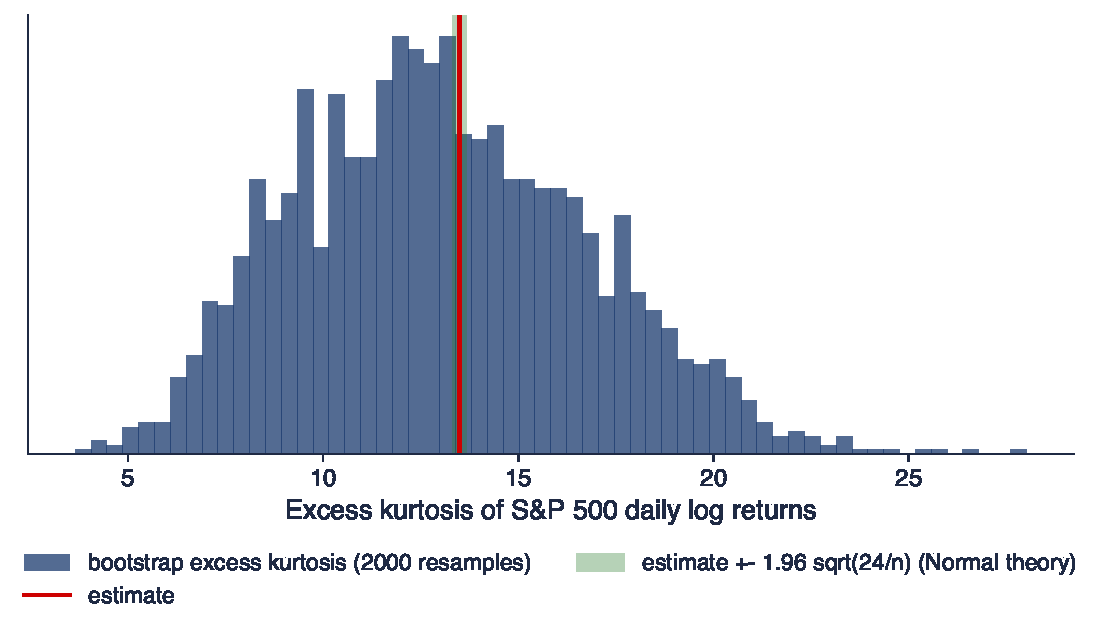
\includegraphics[width=1.0\textwidth,height=0.55\textheight,keepaspectratio]{ch2_sem_b1.pdf}
\end{center}
\vspace{-2mm}

\end{column}
\begin{column}{0.50\textwidth}
\begin{itemize}
    \item $n = 4\,201$; mean $0.045\%$, s.d. $1.08\%$; worst day $-12.8\%$ on 16 March 2020
    \item $S = -0.61$ (SE $0.038$), $K = 13.49$ (SE $0.076$); $\text{JB} = 32\,113$: normality rejected
    \item Normal theory: $K \in [13.34, 13.64]$; bootstrap: $[6.7, 20.6]$; for $S$, bootstrap $[-1.54, 0.29]$
    \item Interpretation: $\sqrt{24/n}$ assumes Normal data; with heavy tails $K$ depends on a few days, and whether they are resampled moves it a lot; the bootstrap s.d. of $K$ is 50 times larger
    \item The skewness interval contains 0: the sign of $S$ is not certain
\end{itemize}
\end{column}
\end{columns}\sfmquantlet{Ch_02}{SFM_ch2_seminar}
\end{frame}

\begin{frame}{B2: Three More Series [Proposed]}
\itemsize{\footnotesize}
\begin{itemize}
\item \textbf{Question}: which of the BET, Bitcoin and OMV Petrom is farthest from the Normal distribution, and how much does one day matter?
\item \textbf{Inputs}: daily log returns, 2010--2026 (Bitcoin from 2014), each on its own calendar; model: B1
\item \textbf{Tasks}
\begin{enumerate}
    \item Compute $n$, mean, standard deviation, $S$, $K$ and JB for each series.
    \item Remove the single largest absolute return of each series and recompute $K$.
    \item Interpretation: what does the change in $K$ tell you about kurtosis as a summary of risk?
\end{enumerate}
\item \textbf{Report}: one table and two sentences
\item Notebook: section B2
\end{itemize}
\end{frame}

\ifsolutions
\begin{frame}{B2: Solution [Proposed]}
\itemsize{\footnotesize}
\begin{center}
\footnotesize
\begin{tabular}{lrrrrrrr}
\toprule
Series & $n$ & Mean & S.d. & $S$ & $K$ & JB & $K$ without max \\
\midrule
BET & 4\,186 & $0.046$ & $1.07$ & $-0.98$ & $17.9$ & 56\,762 & $15.3$ \\
Bitcoin & 4\,384 & $0.118$ & $3.49$ & $-0.70$ & $12.0$ & 26\,482 & $5.3$ \\
OMV Petrom & 3\,815 & $0.076$ & $1.62$ & $-0.54$ & $8.9$ & 12\,832 & $7.0$ \\
\bottomrule
\end{tabular}
\end{center}
\begin{itemize}
    \item Removed days: BET 19 December 2018 ($-11.9\%$), Bitcoin 12 March 2020 ($-46.5\%$), SNP 25 May 2010 ($-15.8\%$)
    \item Farthest from the Normal distribution by $K$ and JB: the BET; all three rejected
    \item Interpretation: one day out of thousands moves the kurtosis of Bitcoin from 12.0 to 5.3; $K$ is a fragile summary, report it with the extremes
\end{itemize}\sfmquantlet{Ch_02}{SFM_ch2_seminar}
\end{frame}
\fi

\begin{frame}{B3: Normal or Student-$t$ for the BET? [Solved]}
\itemsize{\footnotesize}
\begin{itemize}
\item \textbf{Question}: does a Student-$t$ describe the daily returns of the BET better than the Normal distribution, and where does each fail?
\item \textbf{Inputs}: BET closes, 2010--2026, daily log returns in \%
\item \textbf{Tasks}
\begin{enumerate}
    \item Draw the QQ plot of the standardised returns against $N(0,1)$.
    \item Fit a Student-$t$ by maximum likelihood and draw the QQ plot against the fitted $t$.
    \item Compare the log-likelihoods and the AIC of the two models.
    \item Interpretation: where does the Normal distribution fail, and where does the fitted $t$ fail?
\end{enumerate}
\item \textbf{Report}: $\hat\nu$, $\hat m$, $\hat s$, two AIC values, two QQ plots, one sentence
\item Notebook: section B3
\end{itemize}
\end{frame}

\begin{frame}{B3: Solution [Solved]}
\itemsize{\scriptsize}
\begin{columns}[T]
\begin{column}{0.50\textwidth}
\begin{center}
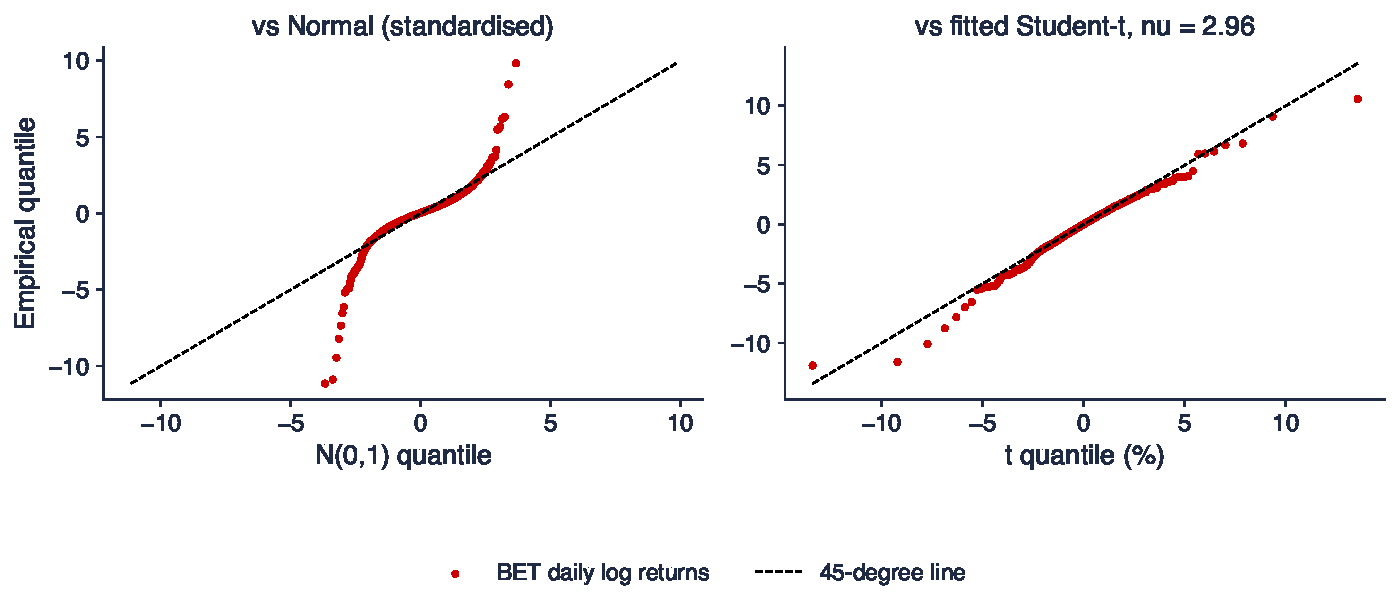
\includegraphics[width=1.0\textwidth,height=0.55\textheight,keepaspectratio]{ch2_sem_b3.pdf}
\end{center}
\vspace{-2mm}

\end{column}
\begin{column}{0.48\textwidth}
\begin{itemize}
    \item $\hat\nu = 2.96$, $\hat m = 0.078\%$, $\hat s = 0.628\%$; implied s.d. $\hat s\sqrt{\hat\nu/(\hat\nu - 2)} = 1.10\%$
    \item $\ell_t = -5496$ vs $\ell_N = -6224$; $\text{AIC}_N - \text{AIC}_t = 1454$: the $t$ wins clearly
    \item Lowest return $-11.9\%$; matching quantile: Normal distribution $-3.9\%$, fitted $t$ $-13.4\%$
    \item Interpretation: the Normal distribution misses both tails (S-shape); the $t$ fits the centre and most of the tails, but its extreme quantiles go slightly beyond the data
\end{itemize}
\end{column}
\end{columns}\sfmquantlet{Ch_02}{SFM_ch2_seminar}
\end{frame}

\begin{frame}{B4: How Many 4-Sigma Days? [Proposed]}
\itemsize{\footnotesize}
\begin{itemize}
\item \textbf{Question}: how many 4-sigma days do the S\&P 500, DAX, BET and Bitcoin have, and which model predicts the count?
\item \textbf{Inputs}: daily log returns, 2010--2026 (Bitcoin from 2014); model: B3
\item \textbf{Tasks}
\begin{enumerate}
    \item Count the days with $|r_t - \bar r| > 4s$ in each series.
    \item Compute the expected count under the Normal distribution and the Poisson probability of seeing at least the observed count.
    \item Compute the expected count under the fitted Student-$t$ (same threshold $\bar r \pm 4s$).
    \item Interpretation: is the Student-$t$ too heavy, too light or about right for each series?
\end{enumerate}
\item \textbf{Report}: one table and one sentence per series
\item Notebook: section B4
\end{itemize}
\end{frame}

\ifsolutions
\begin{frame}{B4: Solution [Proposed]}
\itemsize{\footnotesize}
\begin{center}
\footnotesize
\begin{tabular}{lrrrrrr}
\toprule
Series & $n$ & observed & Normal & $p$ (Poisson) & $\hat\nu$ & Student-$t$ \\
\midrule
S\&P 500 & 4\,201 & 28 & $0.27$ & ${2 \times 10^{-46}}$ & $2.78$ & $34.9$ \\
DAX & 4\,244 & 20 & $0.27$ & ${1 \times 10^{-30}}$ & $3.31$ & $29.5$ \\
BET & 4\,186 & 28 & $0.27$ & ${2 \times 10^{-46}}$ & $2.96$ & $28.1$ \\
Bitcoin & 4\,384 & 29 & $0.28$ & ${6 \times 10^{-48}}$ & $2.23$ & $54.8$ \\
\bottomrule
\end{tabular}
\end{center}
\begin{itemize}
    \item The Normal distribution is rejected for every series: the observed counts are 74--106 times the expected ones
    \item Interpretation: the $t$ is about right for the BET, somewhat too heavy for the S\&P 500 and the DAX, and much too heavy for Bitcoin ($\hat\nu$ close to 2)
    \item One $\nu$ fits the whole distribution by likelihood, which is dominated by the many ordinary days, not by the few extreme ones
\end{itemize}\sfmquantlet{Ch_02}{SFM_ch2_seminar}
\end{frame}
\fi

\begin{frame}{B5: Does the S\&P 500 Become Normal at Longer Horizons? [Solved]}
\itemsize{\footnotesize}
\begin{itemize}
\item \textbf{Question}: are 5-day and 21-day returns of the S\&P 500 closer to the Normal distribution than daily returns?
\item \textbf{Inputs}: S\&P 500 daily log returns, 2010--2026; $h$-day returns are sums over non-overlapping blocks of $h$ days
\item \textbf{Tasks}
\begin{enumerate}
    \item Build the 5-day and 21-day log returns.
    \item Compute $n$, $S$, $K$, the standard error $\sqrt{24/n}$ and JB with its $p$-value at $h = 1, 5, 21$.
    \item Draw the three QQ plots against $N(0,1)$.
    \item Interpretation: is the monthly distribution Normal, and why does the test have less power at $h = 21$?
\end{enumerate}
\item \textbf{Report}: a table with three rows, three QQ plots, two sentences
\item Notebook: section B5
\end{itemize}
\end{frame}

\begin{frame}{B5: Solution [Solved]}
\itemsize{\scriptsize}
\begin{center}
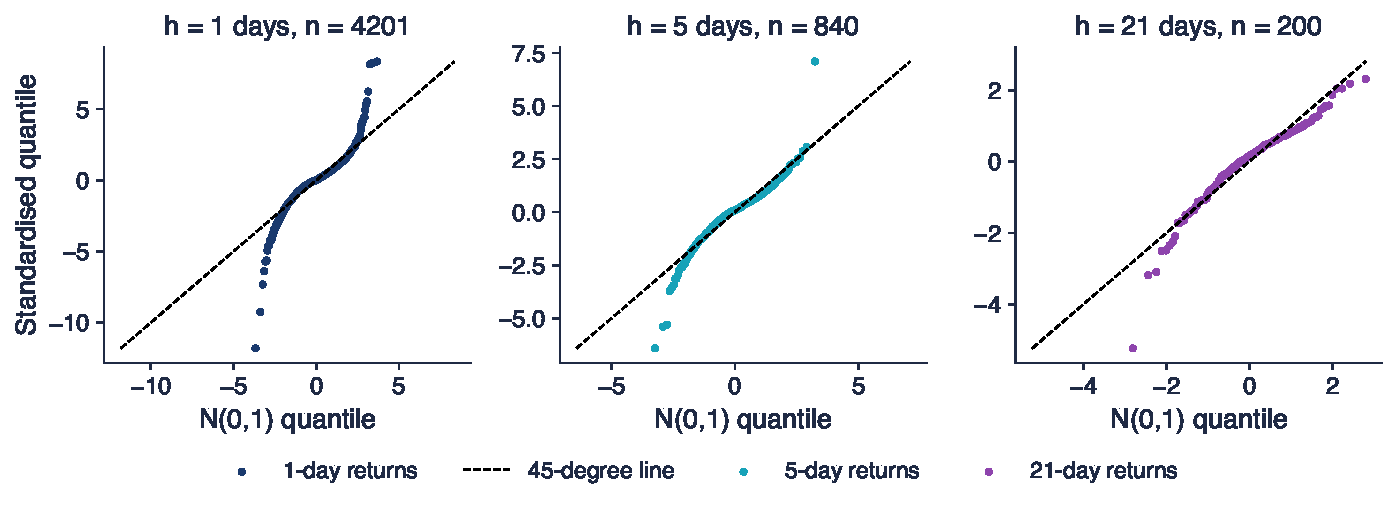
\includegraphics[width=0.96\textwidth,height=0.42\textheight,keepaspectratio]{ch2_sem_b5.pdf}
\end{center}
\vspace{-2mm}
\begin{center}
\scriptsize
\begin{tabular}{rrrrrr}
\toprule
$h$ & $n$ & $S$ & $K$ & $\sqrt{24/n}$ & JB ($p$) \\
\midrule
1 & 4201 & $-0.61$ & $13.49$ & $0.08$ & 32\,113 (${\approx 0}$) \\
5 & 840 & $-0.62$ & $7.06$ & $0.17$ & 1\,797 (${\approx 0}$) \\
21 & 200 & $-1.18$ & $3.68$ & $0.35$ & 159 (${2.9 \times 10^{-35}}$) \\
\bottomrule
\end{tabular}
\end{center}
\begin{itemize}
    \item Interpretation: $K$ falls from 13.49 to 3.68, but monthly returns are still not Normal (skewness $-1.18$, March 2020); with only 200 months, the standard error of $K$ is 0.35, so smaller departures would go undetected
\end{itemize}\sfmquantlet{Ch_02}{SFM_ch2_seminar}
\end{frame}

\begin{frame}{B6: Are BET Returns Independent? [Proposed]}
\itemsize{\footnotesize}
\begin{itemize}
\item \textbf{Question}: are the daily returns of the BET uncorrelated, and are they independent?
\item \textbf{Inputs}: BET daily log returns, 2010--2026; model: B5
\item \textbf{Tasks}
\begin{enumerate}
    \item Compute the ACF of $r_t$ and of $|r_t|$ at lags 1--10 and the band $\pm 1.96/\sqrt n$.
    \item Compute the Ljung--Box statistic $Q(10)$ for $r_t$ and for $|r_t|$ and compare with $\chi^2_{0.95}(10)$.
    \item Interpretation: can returns be uncorrelated but not independent?
\end{enumerate}
\item \textbf{Report}: two ACF columns, two $Q$ values, one sentence
\item Notebook: section B6
\end{itemize}
\end{frame}

\ifsolutions
\begin{frame}{B6: Solution [Proposed]}
\itemsize{\footnotesize}
\begin{itemize}
    \item $n = 4\,186$, band $\pm 0.030$
    \item $r_t$: $\hat\rho(1), \hat\rho(2), \hat\rho(3) = 0.034, 0.056, -0.018$; 5 of 10 lags outside the band; $Q(10) = 45.7$ ($p = 1.6 \times 10^{-6}$)
    \item $|r_t|$: $0.335, 0.241, 0.260$, \dots, $0.201$ at lag 10; $Q(10) = 2120$, far above $18.31$
    \item The test on $r_t$ also rejects, but the autocorrelations are at most 0.06 in absolute value and the band assumes i.i.d. data, which volatility clustering violates
    \item Interpretation: yes; independence would make $|r_t|$ uncorrelated too; the strong autocorrelation of $|r_t|$ shows that the size of returns is predictable, their sign much less
\end{itemize}\sfmquantlet{Ch_02}{SFM_ch2_seminar}
\end{frame}
\fi

\begin{frame}{B7: Is Bitcoin Like a Stock Index? [Proposed]}
\itemsize{\footnotesize}
\begin{itemize}
\item \textbf{Question}: do the S\&P 500 and Bitcoin both show the leverage effect and the gain/loss asymmetry?
\item \textbf{Inputs}: daily log returns, S\&P 500 2010--2026, Bitcoin 2014--2026; model: B5
\item \textbf{Tasks}
\begin{enumerate}
    \item Compute $L(k) = \text{Corr}(r_t, |r_{t+k}|)$ for $k = 1, \dots, 5$ and their mean, with the band $\pm 1.96/\sqrt n$.
    \item Count the days below $\bar r - 4s$ and above $\bar r + 4s$; test whether falls and rises are equally likely (binomial test, $p = 0.5$).
    \item Compare $|q_{0.01}|$ and $q_{0.99}$ and the skewness.
    \item Interpretation: which stylised facts of stock indices does Bitcoin share?
\end{enumerate}
\item \textbf{Report}: one table and two sentences
\item Notebook: section B7
\end{itemize}
\end{frame}

\ifsolutions
\begin{frame}{B7: Solution [Proposed]}
\itemsize{\footnotesize}
\begin{center}
\footnotesize
\begin{tabular}{lrrrrrrrr}
\toprule
Series & $L(1)$ & $\bar L(1..5)$ & band & $< -4s$ & $> +4s$ & $p$ & $|q_{0.01}|$ & $q_{0.99}$ \\
\midrule
S\&P 500 & $-0.122$ & $-0.121$ & $0.030$ & 16 & 12 & $0.57$ & $3.15$ & $2.61$ \\
Bitcoin & $-0.073$ & $-0.031$ & $0.030$ & 18 & 11 & $0.26$ & $10.51$ & $9.87$ \\
\bottomrule
\end{tabular}
\end{center}
\begin{itemize}
    \item Leverage: clear for the S\&P 500 ($\bar L = -0.121$, 4 times the band); for Bitcoin only at lag 1, the mean is at the edge of the band
    \item More extreme falls than rises in both, but with so few extreme days the binomial test cannot reject equality ($p = 0.57$ and $0.26$)
    \item Interpretation: Bitcoin shares heavy tails, clustering and negative skewness ($-0.70$), but the leverage effect is weak: there is no firm with debt behind it
\end{itemize}\sfmquantlet{Ch_02}{SFM_ch2_seminar}
\end{frame}
\fi


%=============================================================================
\section{Part C: Open Questions and AI Critique}
%=============================================================================

\begin{frame}{C1: Are Bitcoin's Tails Getting Thinner? [Proposed]}
\itemsize{\footnotesize}
\begin{itemize}
\item \textbf{Question}: has the tail of Bitcoin's daily returns become thinner since 2015, as its market matured?
\item \textbf{Inputs}: Bitcoin and S\&P 500 daily log returns, 2015--2026; models: B3, B5
\item \textbf{Tasks}
\begin{enumerate}
    \item Fit a Student-$t$ and compute the excess kurtosis for each calendar year and each series.
    \item Compute the Spearman rank correlation between the year and $\hat\nu$.
    \item Fit one $t$ on 2015--2020 and one on 2021--2026 and compare $\hat\nu$.
    \item Propose one way to make the answer more reliable (intervals, other windows, other crypto assets).
    \item Interpretation: what can 12 yearly estimates tell us about a trend?
\end{enumerate}
\item \textbf{Report}: a table, the rank correlation with its $p$-value, a short plan for a project
\item Notebook: section C1
\end{itemize}
\end{frame}

\ifsolutions
\begin{frame}{C1: Reference Analysis [Proposed]}
\itemsize{\footnotesize}
\begin{itemize}
    \item Bitcoin: yearly $\hat\nu$ between 1.5 and 5.1; Spearman with the year $0.63$ ($p = 0.03$, 12 years)
    \item Two halves: $\hat\nu$ = 1.91 (2015--2020) and 2.69 (2021--2026)
    \item S\&P 500: Spearman $0.31$ ($p = 0.32$); $\hat\nu$ = 2.13 and 4.06: the benchmark also changed
    \item Weak evidence of thinner Bitcoin tails, but one test on 12 noisy points, chosen after seeing the data; calm years alone can raise $\hat\nu$
    \item Project directions: rolling windows with bootstrap intervals, returns scaled by a rolling volatility, Ethereum and Solana, the Hill estimator of Chapter 5
\end{itemize}\sfmquantlet{Ch_02}{SFM_ch2_seminar}
\end{frame}
\fi

\begin{frame}{C2: Audit an AI Answer [Proposed]}
\itemsize{\scriptsize}
\begin{itemize}
    \item A student asked an AI assistant: ``Describe the distribution of daily S\&P 500 returns in 2010--2026.'' The answer:
    \item \aiprompt{(a) The excess kurtosis is 13.5; since the Normal distribution has kurtosis 0, the kurtosis of the S\&P 500 is 13.5.}
    \item \aiprompt{(b) JB = 32\,113 with p = 0.000, which proves that the returns follow a Student-t distribution.}
    \item \aiprompt{(c) A Normal 4-sigma day happens once every 15\,787 days; the 28 such days in 4\,201 days are just bad luck.}
    \item \aiprompt{(d) The lag-1 autocorrelation is only -0.11, so returns are independent and volatility cannot be predicted.}
    \item \aiprompt{(e) With yearly log returns N(7\%, 18\%\textasciicircum 2), the expected value of 100 invested after one year is 100 exp(0.07) = 107.25.}
    \item Tasks
    \begin{itemize}
        \item 1. For each statement, say whether it is correct; if not, give the correct statement and the correct number from the notebook (section C2).
        \item 2. Report: a list of five verdicts with one line of justification each.
    \end{itemize}
\end{itemize}
\end{frame}

\ifsolutions
\begin{frame}{C2: Solution [Proposed]}
\itemsize{\footnotesize}
\begin{itemize}
    \item (a) Wrong: the Normal kurtosis is 3 (excess 0); kurtosis $= 13.5 + 3 = 16.5$
    \item (b) Wrong: JB only rejects normality; the fitted $t$ ($\hat\nu = 2.78$) is better by AIC, but its QQ plot still misses the extremes and it is symmetric
    \item (c) Wrong: the Normal expectation is $0.27$ days; seeing 28 has Poisson probability about $2 \times 10^{-46}$: the model is wrong, not the luck
    \item (d) Wrong: uncorrelated is not independent; the ACF of $|r_t|$ is $0.31$ at lag 1 and $0.26$ at lag 10, Ljung--Box $Q(10) = 3859$: volatility is predictable
    \item (e) Wrong: $100e^{0.07} = 107.25$ is the median; the mean is $100e^{0.07 + 0.18^2/2} = 109.00$
\end{itemize}\sfmquantlet{Ch_02}{SFM_ch2_seminar}
\end{frame}
\fi


%=============================================================================
\section{Wrap-Up}
%=============================================================================

\begin{frame}{What You Should Take from Today}
\itemsize{\small}
\begin{itemize}
    \item The Normal distribution makes 4-sigma days almost impossible; real markets have them every few months
    \item Lognormal prices: the median is below the mean by the volatility drag
    \item Skewness and kurtosis are fragile: report bootstrap intervals and the extremes
    \item The Student-$t$ fits much better than the Normal distribution, but not perfectly
    \item Returns are nearly uncorrelated but not independent: their size is predictable
    \item An AI answer is a draft: check every definition, model and number
\end{itemize}
\end{frame}

\begin{frame}{After the Seminar}
\itemsize{\small}
\begin{itemize}
    \item Lecture 2 develops each topic of today: the Normal distribution and lognormal models, the CLT, moments and tests, the Student-$t$ and six stylised facts
    \item Try the [Proposed] tasks in the notebook; the solutions are discussed in class
    \item C1 can grow into a team project: rolling windows, bootstrap intervals, more crypto assets
    \item Reading: \refFHH, Sec.~3.3 and Sec.~11.2; exercises with solutions: \refFHHex
\end{itemize}
\end{frame}


%=============================================================================
\section{References}
%=============================================================================

\begin{frame}{References}
\itemsize{\tiny}
\begin{itemize}
    \item Borak, S., Härdle, W.K., López-Cabrera, B. (2013). \href{https://doi.org/10.1007/978-3-642-33929-5}{\textit{Statistics of Financial Markets: Exercises and Solutions}}, 2nd ed. Springer.
    \item Cont, R. (2001). \href{https://doi.org/10.1080/713665670}{Empirical properties of asset returns: stylized facts and statistical issues}. \textit{Quantitative Finance}, 1(2), 223--236.
    \item Franke, J., Härdle, W.K., Hafner, C.M. (2019). \href{https://doi.org/10.1007/978-3-030-13751-9}{\textit{Statistics of Financial Markets: An Introduction}}, 5th ed. Springer.
    \item Jarque, C.M., Bera, A.K. (1987). \href{https://doi.org/10.2307/1403192}{A test for normality of observations and regression residuals}. \textit{International Statistical Review}, 55(2), 163--172.
    \item Ljung, G.M., Box, G.E.P. (1978). \href{https://doi.org/10.1093/biomet/65.2.297}{On a measure of lack of fit in time series models}. \textit{Biometrika}, 65(2), 297--303.
    \item Student (1908). \href{https://doi.org/10.1093/biomet/6.1.1}{The probable error of a mean}. \textit{Biometrika}, 6(1), 1--25.
\end{itemize}
\end{frame}

\end{document}
